\documentclass{rspublic}   

%------------------------------------------------------------------------- 
% take the % away on next line to produce the final camera-ready version 
%\pagestyle{empty}

%\usepackage[utf8]{inputenc}
\usepackage{graphicx}
\usepackage{url}
\usepackage{float}
\usepackage{times}    
\usepackage{multirow}    
\usepackage{listings}   
\usepackage{times}     
\usepackage{paralist}    
\usepackage{wrapfig}    
\usepackage[small,it]{caption}
\usepackage{multirow}
\usepackage{ifpdf}   
\usepackage{subfigure} 

                    
%Bibliography                     
\usepackage{natbib}   

\usepackage{listings}
\usepackage{keyval}  
\usepackage{color}
\definecolor{listinggray}{gray}{0.95}
\definecolor{darkgray}{gray}{0.7}
\definecolor{commentgreen}{rgb}{0, 0.4, 0}
\definecolor{darkblue}{rgb}{0, 0, 0.4}
\definecolor{middleblue}{rgb}{0, 0, 0.7}
\definecolor{darkred}{rgb}{0.4, 0, 0}
\definecolor{brown}{rgb}{0.5, 0.5, 0}

\title[Efficient Large-Scale Replica-Exchange Simulations on
Production Infrastructure]{Efficient Large-Scale Replica-Exchange
  Simulations on Production Infrastructure}

\author[Thota, Luckow, Jha]{
  Abhinav Thota$^{1,2}$, Andr\'e Luckow$^{1}$ and Shantenu Jha$^{1,2,3}$\\
  \small{\emph{$^{1}$Center for Computation \& Technology, Louisiana State University, Baton Rouge, LA 70803, USA}}\\
  \small{\emph{$^{2}$Department of Computer Science, Louisiana State
      University, Baton Rouge, LA 70803, USA}}\\
  \small{\emph{$^{3}$e-Science Institute, Edinburgh EH8 9AA, UK}}\\
}

%\date{}

\def\acknowledgementname{Acknowledgements}
\newenvironment{acknowledgement}%
{\section*{\acknowledgementname}%
\parindent=0pt%
}

\newif\ifdraft
\drafttrue
\ifdraft
\newcommand{\jhanote}[1]{ {\textcolor{red} { ***shantenu: #1 }}}
\newcommand{\alnote}[1]{ {\textcolor{blue} { ***andre: #1 }}}
\newcommand{\athotanote}[1]{ {\textcolor{green} { ***athota: #1 }}}
\else
\newcommand{\alnote}[1]{}
\newcommand{\athotanote}[1]{}
\newcommand{\jhanote}[1]{}
\fi

\newcommand{\I}[1]{\textit{#1}}
\newcommand{\B}[1]{\textbf{#1}}
\newcommand{\T}[1]{\texttt{#1}}

\newcommand{\glidein}[1]{Glide-In }  
\newcommand{\ReplicaAgent}[1]{Replica-Agent }         
\newcommand{\replicaagent}[1]{replica-agent }         
\newcommand{\remanager}[1]{RE-Manager }

\begin{document} 


\maketitle    

\begin{abstract}{Replica-Exchange, SAGA, Large-Scale, Production}  

  The design and development of an application is often influenced and
  constrained by the programming systems and the infrastructure it is
  developed against.  It is important to breaking the coupling between
  the development and the underlying infrastructure, in order to
  enable applications to be flexible (across infrastructure),
  extensible (to new methods of communication and coordination) and
  scalable.  Developing applications that are able to orchestrate
  heterogeneous resources across distributed resources is a complex
  task yet is an important design objective of both logically and
  physically distributed applications.  In this work, we focus on the
  Replica-Exchange (RE) Methods which represent a class of algorithms
  that involve a large number of loosely-coupled ensembles and are
  used to understand physical phenomena -- ranging from protein
  folding dynamics to binding affinity calculations.  We develop a
  flexible, extensible and scalable implementation of RE that can
  utilise a range of production cyberinfrastructure concurrently, that
  supports different replica pairing mechanisms (synchronous versus
  asynchronous) and coordination mechanisms, and thereby different
  variants of the RE algorithm. We implement and characterise the
  performance of our implementation at unprecedented scales.

%  flexible and robust implementation enables the efficient use of a
%   broad range of infrastructure.
%   (publish-subscribe centralised notification),

% Developing applications that are able to orchestrate heterogeneous
% resources across distributed resources is a complex task. Inevitably,
% the design and development of an application is influenced and
% constrained by the programming systems and the infrastructure it is
% developed against. Breaking this coupling between the development and
% the underlying infrastructure, to enable applications to be flexible
% (across infrastructure), extensible (to new methods of communication
% and coordination) and scalable is an important design objective of
% distributed applications both logically distributed and physically
% distributed.  In this work, we focus on the Replica-Exchange (RE)
% Methods which represent a class of algorithms that involve a large
% number of loosely-coupled ensembles. RE simulations are used to
% understand physical phenomena Ð ranging from protein folding dynamics
% to binding affinity calculations.  In this work, we develop a
% flexible, extensible and scalable implementation of RE that can
% utilise a range of infrastructure concurrently (and
% autonomically/adaptively), that supports different coordination
% mechanisms (publish/subscribe, centralized notification), different
% replica pairing mechanisms (synchronous versus asynchronous) and
% thereby different variants of the RE algorithm. We implement and
% demonstrate how a flexible and robust implementation enables the
% efficient use of a broad range of infrastructure.

\end{abstract}

\jhanote{Since this is going to Her Majesty's Land, we need to be
  consistent with ``s'' over ``z'' -- organise not organize etc}

\jhanote{In general please don't use hard numbers, but use pointers to
  sections!}
\athotanote{do you mean this: \S\ref{repexfw}}
\jhanote{Not necessary the~\S~but definitely the
  used of ref{sectionlabel} }

\section{Introduction}
Developing applications that are able to orchestrate heterogeneous
resources across distributed resources is a complex task.  Inevitably,
the design and development of an application is influenced and
constrained by the programming systems and the infrastructure it is
developed against. Breaking this coupling between the development and
the underlying infrastructure, to enable applications to be flexible
(across infrastructure), extensible (to new methods of communication
and coordination) and scalable is an important design objective of
distributed applications -- both logically distributed and physically
distributed.

In this work, we focus on the Replica-Exchange
(RE)~\citep{hansmann,Sugita:1999rm} methods -- which represent a class
of algorithms that involve a large number of loosely-coupled
ensembles.  RE simulations are used to understand physical phenomena
-- ranging from protein folding dynamics to binding affinity
calculations. Most RE implementations are either infrastructure
specific (Woods et al. 2005) or, if using multiple distributed
resources, they require prior co-scheduling (Manos et
al. 2008). ~\cite{Luckow:2008fp} takes it to the next level and is an
example of adaptive RE simulations on production-level grid resources,
while ~\cite{parashar_arepex} is an example of \emph{asynchronous} RE
simulations, which is based on
CometG~\citep{Li:2005:CSC:1090948.1091381}, a decentralised
computational infrastructure for Desktop Grid environments.

Application formulations that are scalable while being flexible and
extensible are better suited to using the diverse range of traditional
and hybrid infrastructure (e.g., Grid-Cloud and heterogeneous
resources).  Along with application formulations that facilitate the
flexible utilisation of a range of infrastructure, it is imperative to
have the correct run-time abstractions that support flexible
deployment of these applications.  In support of flexible and scalable
formulations of the RE class of algorithms, we develop a RE Framework
that supports multiple formulations, is extensible to a broad range of
infrastructure and as we shall show is scales-up and scales-out.

Our RE Framework utilises a flexible pilot-job implementation (SAGA
BigJob) to support the execution of the ensembles.  It supports
scalable implementation of RE that can utilize a range of
infrastructure concurrently that supports different coordination
mechanisms (publish-subscribe, centralised notification), different
replica pairing mechanisms (synchronous versus asynchronous) and
thereby different variants of the RE algorithm.  We compare and
analyze the performance of the different RE formulations (synchronous
and asynchronous) when scaled-up to 256 replicas, and scaled-out to 4
machines. % \jhanote{Last sentence is unclear} We present results using
% which the reader can understand which model of RE is most suited for a
% particular set of resources (distributed, local etc.,)

The paper is organised as follows. Section~\ref{sec:repex-approach}
sketches out the three different RE algorithms that are investigated; 
we also present an approximate mathematical model for the different algorithms.  
Section~\ref{repexfw} outlines the architecture of the RE Framework -- the SAGA BigJob
(how it supports the dynamic execution of multiple replicas) and other
important elements that make the framework flexible and extensible.
In section~\ref{sec:re_impl}, we present our implementation of the RE algorithms and
understand the primary determinants of performance and relate it to
the mathematical model of section~\ref{sec:repex-approach}.  
In section~\ref{sec:performance}, we describe the experiments performed 
to assess and understand performance when scaling-up (on a single machine) 
as the number of replicas increases. We also investigate the scaling-out
characteristics, namely performance as the number of replicas are
increased while the (distributed) resources employed
increases. % while keeping the number of replicas on local and
% distributed resources.  \jhanote{Currently we have only Section 6
%   and no 7}.
% We present the results and analysis, in Section VI and 
Section~\ref{sec:conclusion} concludes the paper and discusses future work.

% \alnote{Should we add a section with some scientific background: HIV,
%   Hepatitis...?}  \jhanote{given the tightness of space, I think we
%   should try to avoid it. OK?}

\section{Replica-Exchange Algorithms}\label{sec:repex-approach}

The RE class of algorithms involve the concurrent execution of
\emph{replicas} - which are defined as instances of essentially
similar simulations but with minor differences, such as the defining
temperature of the replica. These replicas are loosely coupled, in
that there is an infrequent exchange between pairs of 
% \jhanote{do we want to say paired?} \athotanote{fixed}
replicas; in addition to the frequency of communication between the
replicas being low (relative to within a single replica), the amount
of information/data exchanged between replicas is small (relative to
the operating data-set size).

% \alnote{We should give a number for $\eta$ for sync
%   RE}\athotanote{wouldn't that be implementation dependent?}
% \alnote{What is the value of $\eta$ for async RE?} \athotanote{as
%   mentioned earlier, i the value depends on the implementation;
%   centralised=1, decentralised= $N_R\over2$} \athotanote{do we need
%   the equation here again?}  \athotanote{I think
%   $\eta_{sync,async-cent}$ should be 1 as only one exchange is done at
%   a time(single master process) and $\eta_{async-decent}$ should be
%   $N_R \over 2$, as each pair is involved in negotiating an
%   exchange. since this depends on implementation, i am not including
%   the $\eta$ values here.} \jhanote{Andre: If the points in the above
%   exchange have been addressed, could you please comment out? Thanks.}

\subsection{Mathematical Model}
\label{sec:math-model}
In the this subsection we develop a mathematical model that captures
the primary components that make up the total runtime of a RE
experiment. In an ideal scenario, the total time to complete an
experiment would be equal to the concurrent runtime of the ensemble of
replicas and there would be no overhead associated with the
coordination of the replicas.  If the ensemble contains $N_R$
replicas, the total number of pairwise exchanges is $N_X$ and the
runtime of a replica to complete a defined number of time steps is
$T_{MD}$, then the total time to complete the RE experiment, $T$ would
be:
\begin{eqnarray}
T = {1\over p} \times (T_{MD} \times  {N_X \over {N_R \over 2}}) 
\label{eq:totaltime}
\end{eqnarray}
where, p is defined as the probability of a successful exchange be $p$
(the probability of a successful exchange is not 1, the
decision to accept an exchange or not is made using the
Metropolis scheme~\citep{metropolis:1087}). However, any RE experiment will entail an overhead
of coordination, job-submission \& termination etc. Thus, the time $T$
to complete the RE experiment where N$_X$ is the total number of
exchanges is:
%\alnote{I would propose to write $\frac{N_X}{\eta}$ to have both terms consistent}
\begin{eqnarray}
  T = {1\over p} \times [(T_{MD} \times  {N_X \over {\eta}}) +
  {(T_{X} + T_{W})} \times {N_X \over \eta}]
\label{eq:totaltime}
\end{eqnarray}
where, $T_{X}$ is the time to perform a pairwise exchange and includes
the following components, (i) time to find a partner ($T_f$), (ii)
time to exchange/write/transfer files ($T_{ex}$) as well as (iii)
book-keeping associated with replica pairing/exchanging ($T_{coord}$)
(thus $T_{X} = T_{f} + T_{ex}+T_{coord}$); 
%\alnote{Do we need to split up$T_{W}$? I don't see a (ii).}
$T_W$ is comprised of the time spent by a replica waiting for other
replicas to become available ($T_w$), the time spent waiting to be restarted
after each exchange ($T_r$) and any other associated costs, and $\eta$
is the number of independent exchange events occurring concurrently,
As we will establish, the coordination and waiting costs differ for
the different RE algorithms.

\subsection{Synchronous Replica Exchange}

Traditionally, RE algorithms have been implemented such that the
exchanges have been synchronous.  If the number of replicas is
${N_R}$, this leads to a {\it fixed} number of ${N_R \over 2}$ pairs
of replicas are created.  When \emph{all} the replicas in the ensemble
reach a pre-determined state (e.g. the Molecular Dynamics (MD)
simulation completes a pre-determined number of steps), an exchange of
temperatures between the paired replicas is attempted using the
Metropolis scheme.  If the exchange attempt is successful, parameters
such as the temperature are swapped.

% In Equation~\ref{eq:totaltime}, we introduced the various components
% that make up the total time to complete an RE experiment. Only 
% 1 para limitation on traditional replica exchange
%running concurrently

For synchronous RE formulation, all replicas must reach a
pre-determined state ({\texttt DONE}), before exchanges are performed.
$T_W$ includes the time waiting for all the replicas in the ensemble
to reach this state, the time spent waiting before the replicas are
restarted after each exchange and any other miscellaneous costs.

A major limitation of this model is that replicas are paired in fixed
groups and thus exchanges take place between pre-determined pairs of
replicas.  As a consequence, of pairs being determined before an
exchange, although $T_f$ is $0$, this limits the number of possible
exchange partners that are available for a given replica; this
inhibits exchanges between replicas with non-nearest temperatures, and
ultimately negates the possibility of crosswalks -- where a crosswalk
is said to occur when a replica originally with a low temperature
reaches the upper temperature range and then returns to the lower
temperature range.

In addition to limitations in modeling the physics, there are rigid
replica-pairing is efficient only in homogeneous environments; for
heterogeneous environments \& systems, where resource availability and
performance fluctuates, the need for synchronisation leads to
slow-down \& inefficiencies. We show how these limitations are
overcome in the asynchronous (exchange) formulations of RE.

\subsection{Asynchronous Replica Exchange}

% - Introduce asynchronous Replica Exchange -- 1 para on case II and
% case III (algorithmically) To overcome these limitations and
% implement çit on distributed grid resources.

In asynchronous formulations of the RE
algorithms~\citep{parashar_arepex,DBLP:journals/jcc/GallicchioLP08}, a
replica does not have to wait for {\it all} other replicas to reach a
pre-determined state. An exchange occurs whenever a replica reaches a
pre-determined state and perform an exchange with another suitable
replica in the ensemble.  The reduction in {\it synchronization}
(wait) times comes at the cost of increased {\it coordination} costs.
The specific values of the terms $T_{X}$ and $T_W$, in
Equation\ref{eq:totaltime} differ from the synchronous formulations.
Since each replica on completing a run has to find a {\it new}
partner, $T_f \neq 0$.  Additionally, $T_W$ only includes the time
spent waiting for the next replica to become available, any time spent
waiting before the replicas are restarted after an exchange and any
other miscellaneous costs.

% a pair of replicas are available, and where \jhanote{Is the
%   algorithm similar or identical? If it is not identical, how is it
%   different, or is it just the case that the implementation is
%   different?} \athotanote{is it ok now? i think we are taking the
%   async algorithm as is and implementing it on production
%   infrastructure. ?}
% Let us look at how the ŧō and waiting costs introduced in
% equation \ref{eq:totaltime2} behave. 

% \alnote{This is too general.  We should drop the redundancy of
%   explaining every component and rather analyze the differences.}
% \athotanote{you are right; i am adding a couple of lines here. does
%   it help?} \jhanote{As currently written, $T_W$ has not been
%   defined or ``different components'' discussed, i.e., this
%   paragraph should come after the modelling section}

% But also, an asynchronous RE algorithm has the potential to perform
% better than the traditional RE: (i) when we scale-up the number of
% replicas and (ii) when we scale-out across many machines.
%\jhanote{There is no basis for this sentence at the moment. REMOVE}

\section{Replica-Exchange Framework}\label{repexfw}

An important motivation for this work is to design and implement a
framework that provides the capability to implement and compare the
performance of the different RE algorithms formulations at
large-scales.  In addition, it is important that framework be
independent of the underlying infrastructure.  It is useful to
highlight that we differ from other RE implementations (e.g.
\cite{parashar_arepex}) in that we use {\it production grade}
national and regional cyberinfrastructure, such as the US TeraGrid and
LONI~\citep{LONI_web}, using general purpose and standard
capabilities.  Additionally, our framework {\it natively} supports
individual replicas that are MPI jobs. In this section we outline the
architecture, implementation and the basic performance of the RE
framework when used to implement the different formulations.

% In following subsections we
% introduce the different components in the RE Framework.

% is to present an infrastructure independent solution that makes it
% possible to implement a variety of RE algorithms, such as synchronous
% and asynchronous, that can
% asynchronous RE model we developed runs on production level grids such
% as the Teragrid, unlike specialized
% infrastructures.

\subsection{SAGA BigJob - A Pilot-job Framework}
\label{sec:BigJob}

% The Simple API for Grid Applications (SAGA)(~\citep{saga_gfd90}) is an
% API that provides the basic functionality required to build
% distributed applications, tools and frameworks so as to be independent
% of the details of the underlying infrastructure. SAGA is an API
% standardization effort within the Open Grid Forum
% (OGF)~\citep{ogf_web}, an international standards development body
% concerned primarily with standards for distributed computing. 

%%%%% FIGURE %%%%%
\begin{figure}[t]
      \centering
          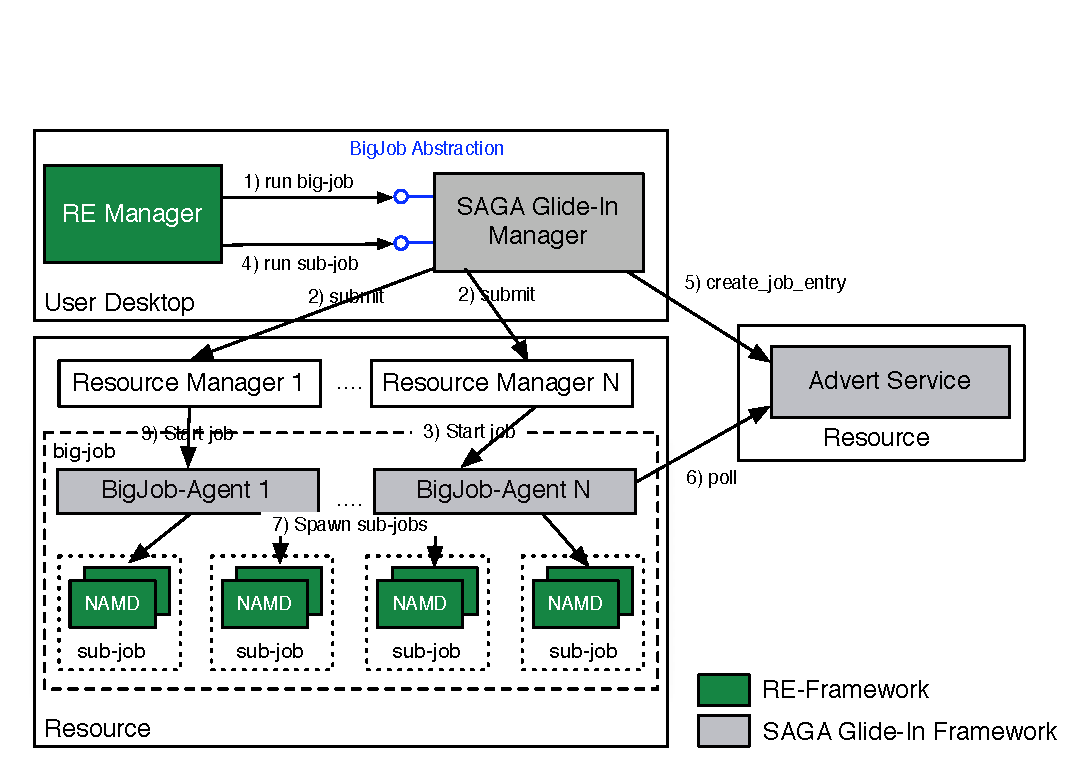
\includegraphics[width=0.82\textwidth]{../figures/Bigjob_arch.pdf}
          \caption{\footnotesize SAGA/BigJob Architecture
              }
      \label{fig:bigjob}
\end{figure}

We have demonstrated the usage of the SAGA-based Pilot-Job
framework~\citep{saga_bigjob_condor_cloud} -- called the BigJob, to
run RE simulations across multiple, heterogeneous, distributed grid
and cloud infrastructure~\citep{Luckow:2008fp}.  SAGA~\citep{saga-url}
is an API to the basic functionality required to build distributed
applications, tools and frameworks so as to be independent of the
details of the underlying infrastructure.  The various tasks that are
carried out using the SAGA APIs include file staging, job spawning and
the conduction of the exchange attempts.

Here we use the BigJob framework to efficiently request and manage
computational resources for multiple replicas.  Specifically, it
enables the dynamical utilisation a range of infrastructures, i.e., it
supports a scheme that does not depend on a static set of resources
that are pre-defined at the time of workload submission.

Figure ~\ref{fig:bigjob} shows the architecture of SAGA BigJob.  It
consists of three components: (i) the SAGA-BigJob Manager, (ii) the
BigJob Agent and (iii) the advert service which is a central key/value
store which is used for communication between the SAGA-BigJob Manager
and the BigJob agent.  The SAGA-BigJob manager submits the BigJobs to
the resource manager and sub-job descriptions to the advert server.
There is a separate BigJob agent for each BigJob, even if there are
multiple BigJobs on a given machine.  Once a BigJob becomes active,
the BigJob agent retrieves the job descriptions from the advert
server, allocates the required number of nodes and launches the
sub-jobs on each resource. The BigJob agent continuously monitors the
running sub-jobs and updates the sub-job states in the advert
server. Once a sub-job finishes running, the nodes are freed and
marked as available. The BigJob agent periodically polls the advert
server for new jobs.

\subsection{Replica-Exchange Manager}\label{repexmanager} 

% \jhanote{Abhinav: This subsection should help the reader understand
%   the basic and common elements of the RE Framework -- job submission,
%   role of bigjob-agent, replica-agent, replica-exchange manager etc
%   etc} \athotanote{job submission, bigjob agent are explained in 3a. RE-Manager is explained below. replica-agent is touched upon but a more detailed explanation in section 3b(ii)}
  
%   \jhanote{ABHINAV: DEFINE THE ROLE OF RE-MANAGER HERE.  Possibly BIGJOB
%   AGENT here if not in previous subsection.}  \athotanote{please check if it's ok now}
  
The RE-Manager is the master process controlling the different
components of the framework and aspects of the exchanges.  The RE
Manager % is an abstraction that
uses the SAGA BigJob Manager; the actual tasks that the RE-Manager
performs out depend on which RE algorithm is being investigated.  A
replica-agent is a wrapper script that manages an individual
replica  -- starts, facilitates the exchange of that replica,
and restarts it.

% And at the least, it is the SAGA BigJob Manager.  At the most,
% launched in place of the replica. The replica-agent implementation
% where the RE-Manager does a lot of work (a centralized
% implementation). But in an implementation where there is a
% \emph{replica-agent} for every replica, the It should be noted that
% synchronous and asynchronous RE are different algorithms and the
% implementation of same algorithm could be centralized and
% decentralized.

The asynchronous RE algorithm can be implemented using a centralised
or decentralised coordination scheme.  In the former, the RE-Manager
manages all the replicas and performs the exchanges; in the
decentralised coordination implementation, multiple replica-agents
take on that responsibility.  It is worth noting that the synchronous
RE algorithm has centralised coordination scheme.  Interestingly, for
decentralised coordination implementation, the RE-Manager is
functionally similar to the SAGA BigJob Manager.

% Synchronous RE is implemented in a centralised fashion. Centralized
% implementation suits synchronous RE because there is a
% synchronization step at the beginning of each exchange step. But we
% implement asynchronous RE in both centralised and decentralised
% fashions.

% The RE-Manager also creates directories, configuration files and
% stages them to the respective directories.  \alnote{We should focus
%   on the RE part here. The BigJob stuff move to subsec a). This
%   should also remove the redundancy with a)}

\begin{figure}%
\centering
\subfigure[Central]{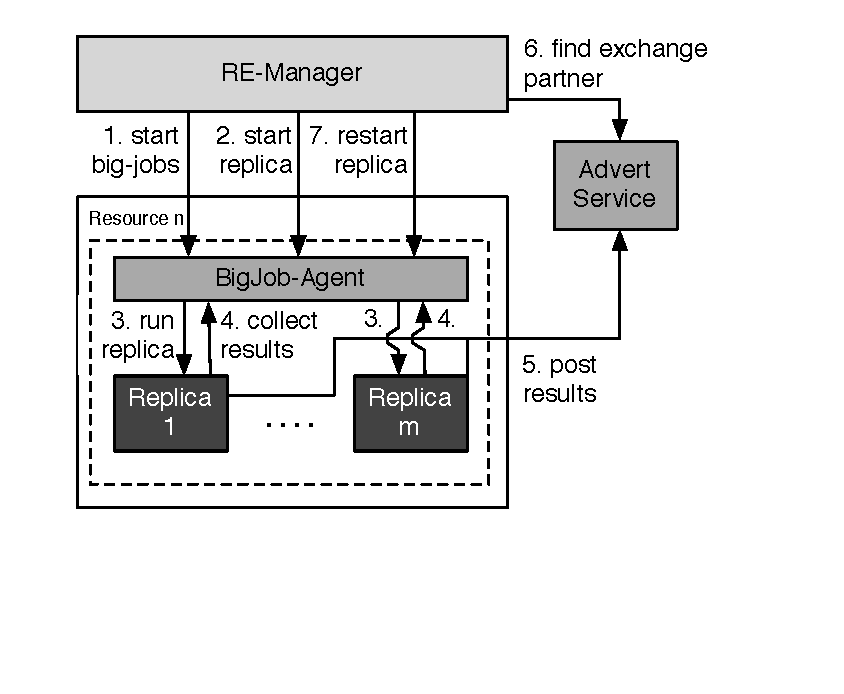
\includegraphics[width=0.47\textwidth]{../figures/central_AL.pdf}}\qquad
\subfigure[Decentral]{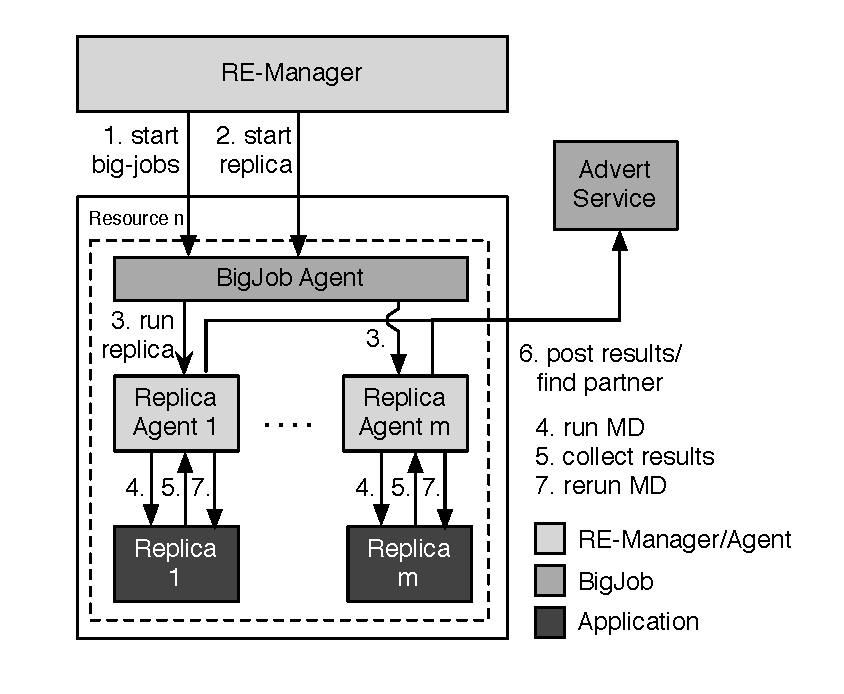
\includegraphics[width=0.47\textwidth]{../figures/decentral_AL.pdf}}\\
\caption{\textbf{Centralised vs. Decentralised Coordination:} Both
  central coordination style is used both by the synchronous RE (case
  I) and a version of the asynchronous RE (case II).  In the decentral
  style -- used by another version of the asynchronous RE (case III)--
  the master is only required for initially setting up all
  replicas. The later coordination is done peer-to-peer via the Advert
  Service.}
\label{fig:coordination}
\end{figure}

% \jhanote{this is an implementation detail. Abhinav: IIUC we restart in
%   both cases -- successful and unsuccessful exchanges. Non? ALso don't
%   toggle between ``replicas'' and ``jobs''!}  

We first explain how the synchronous and asynchronous (centralised) RE
Manager works in the following section followed by an explanation of
how the asynchronous (decentralised) RE-Manager/replica-agent
combination works.

\subsubsection{Synchronous and Asynchronous (centralised) RE-Manager}

% We first explain how the synchronous RE-Manager works and then
% explain asynchronous (centralized) RE-Manager. 
% centralized implementation, Figure~\ref{fig:coordination}a) can be
% used to describe both.

% The architecture of an asynchronous (centralized) RE-Manager is
% similar to that of synchronous RE-Manager.
% Figure~\ref{fig:coordination}a) shows the control flow.

The control flow of a centralised RE scheme is shown in
Figure~\ref{fig:coordination}(a), which can be used to understand both
the asynchronous (centralised) RE and synchronous RE implementations.
Once the BigJobs and replicas are running, the RE-Manager constantly
queries the SAGA BigJob Manager for the latest replica states.  When
the RE-Manager finds a replica that has finished running, it collects
the energy and temperature of that replica by reading the output
file. Once \emph{all} the replicas have finished running, the
RE-Manager performs the exchanges by swapping temperatures and writing
new configuration files. The new configuration files are staged to the
appropriate location. The RE-Manager then submits the replicas for
restarting, and the SAGA BigJob Manager restarts them. The RE-Manager
keeps count of the successful exchanges, until the required number of
exchanges are done.

The implementation of the asynchronous (centralised) RE-Manager, is
different from the synchronous RE-Manager, in that, instead of waiting
for \emph{all} replicas to finish running before performing \emph{all}
exchanges, whenever the asynchronous (centralised) RE-Manager finds a
replica that has finished running, it tries to find a partner to make
an exchange. In order to find a partner, the RE-Manager goes over the
list of all the replicas in the ensemble. If it finds a replica
available it attempts the exchange. If a replica is not found
available, the RE-Manager queries the SAGA BigJob Manager for the
latest replica states and updates its local list. It then loops over
the list to find a replica that has finished running and a partner to
exchange with that replica.  If successful, the replicas are submitted
to be restarted. % \alnote{see comment about BJ
%   impl. detail above}.
% The RE-Manager counts the successful
% exchanges. This process is repeated till all the exchanges are made.


% \alnote{Not sure what we should do with the following paragraph}
% \jhanote{Does not belong here} It should be noted that where as in the
% synchronous RE, the exchanges are conducted when all replicas finish
% running. And the replicas are restarted only after all the exchanges
% are completed. But in an asynchronous (centralized) RE, the exchanges
% are conducted whenever possible and the replicas are restarted.

\subsubsection{Asynchronous (decentralised) RE-Manager and the replica-agent}

% Thus, after the replica-agents are launched, the RE-Manager and the
% SAGA BigJob Manager don't have any responsibilities.
 

Figure~\ref{fig:coordination}(b) shows the asynchronous
(decentralised) RE control-flow.  In the asynchronous (decentralised)
implementation, in order to conduct the exchanges the RE-Manager
launches multiple replica-agents (in lieu of replicas directly).
Replica-agents then take control of replica start/re-start and
exchange attempts.  The replica-agents upon launch, run the replicas;
%\jhanote{what is nodefile? I know what it is but use the
%  general description of what is happening here} 
\alnote{refined} \jhanote{Thanks Andre. Should have been clear, it was
  for Abhinav to understand. Sorry you had to do it} A list of nodes
that is used to carry out the MD run is passed to the replica-agent as
an argument at startup.  The replica-agent constantly monitors the
replica, and when the replica finishes, it updates the advert server
with the current state of that replica.  It also reads the temperature
and energy from the output files, and posts the values to the advert
server.  The RE-Manager is primarily responsible for keeping track and
count of the number of exchanges performed; when the desired number of
exchanges are done, the RE-Manager ends the experiment.

% \jhanote{ISNT THE NEXT PARAGRAPH ESSENTIALLY THE SAME AS THE PREVIOUS
%   PARAGRAHGP? WHY DONT YOU REFER TO THE FIGURE AND THE BASIC StePS
%   OUTLINED IN THE FIGURE?}
  
% \begin{figure}[t] \centering
%           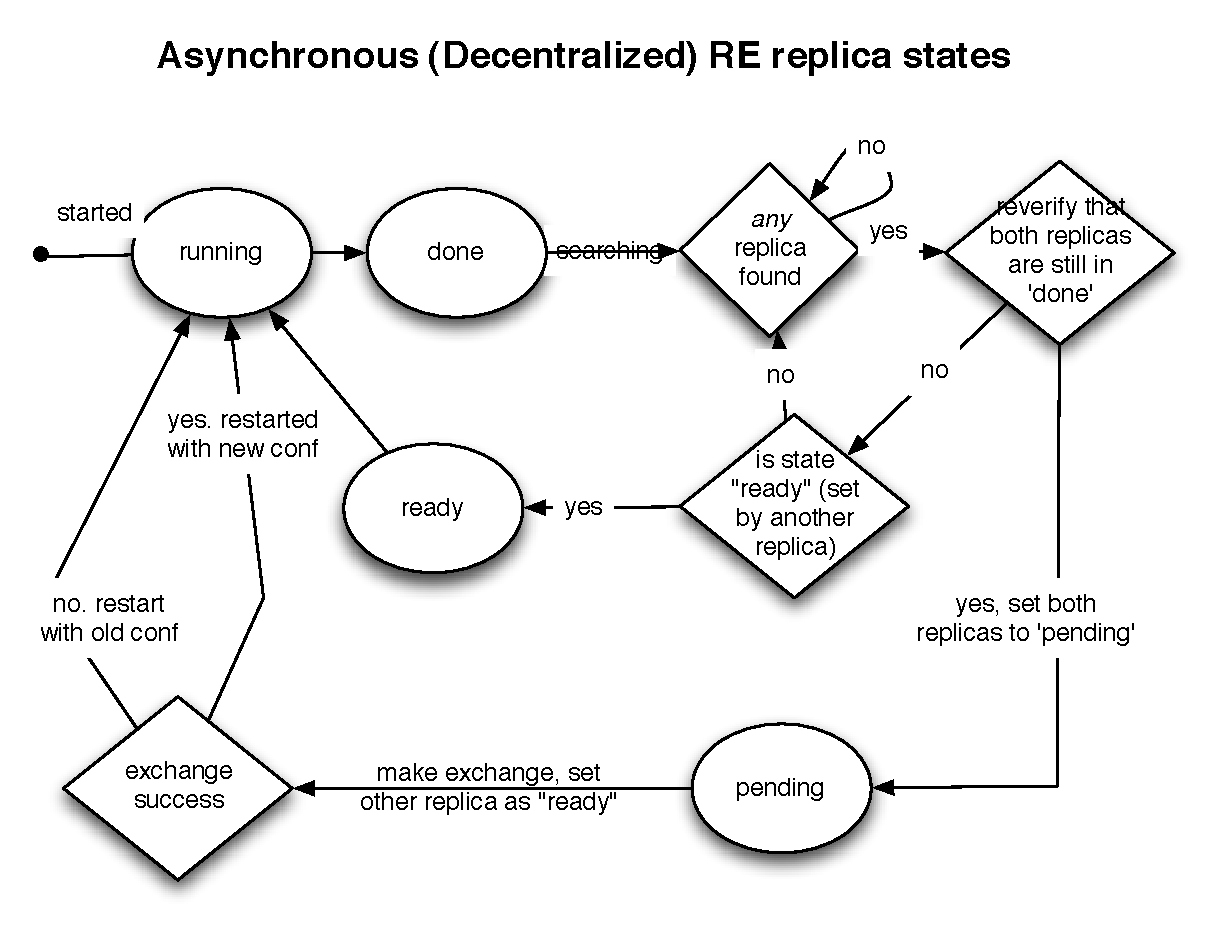
\includegraphics[width=0.82\textwidth]{../figures/decent_state.pdf}
%           \caption{\footnotesize Asynchronous (decentralized) RE
% replica state diagram } \alnote{This chart is not correct yet. There
% can't be state changes on conditional fields} \jhanote{is this a four
% state model or a 3 state model?}
%       \label{fig:state}
% \end{figure}

% As shown in state diagram  (Figure \ref{fig:state}) 
% The replica-agent also goes through the list of replicas randomly to
% try to find an exchange partner.  

% \alnote{In the original state chart we had a ``free'' state. I think
%   this state is needed to ensure the atomicity property of the
%   exchange protocol (2pc style).}
% \jhanote{Would the \texttt{free}
%   state the same as the \texttt{complete} state?}
% \athotanote{i think a replica in \texttt{free} state implies that it
%   is available to make exchanges (meanwhile it also searches or a
%   partner). in the present explanation, that would be \texttt{done}
%   state} 


\jhanote{Are the four states/description common to all RE cases? If
  yes, why is it in this paragraph and not in a subsection that is in
  scope for all three cases? If not, what are the states for the other
  cases?}

A replica can be in one of the three states: (i) \texttt{running},
(ii) \texttt{done}, (iii) \texttt{pending} (for an exchange) and (iv)
\texttt{complete} (exchange has been completed). % \athotanote{after an
%   exchange is complete, the state has to be set as complete by the
%   exchange-initiator, so that the other replica-agent can restart its
%   replica}
When a replica reaches a pre-determined state it (the
replica-agent acts as the proxy for the replica) transitions from
\texttt{running} to \texttt{done}. It initiates the search for a
partner, and scans the list of replicas randomly, so as to avoid
contention if multiple replicas have initiated a search for a
partner. If a replica finds another replica available, it reverifies
their states (to ensure that both replicas are still in \texttt{done}
state), and sets their states as \texttt{pending}. After the exchange
is performed (the temperature of both replicas in the advert server
has been changed), their states are set as \texttt{complete}. Both
replica-agents write new configuration files with the updated
temperatures from the advert server and restart their replicas.

% The search for an exchange partner is conducted in a random
% manner when the number of replicas in the ensemble is large, so as to
% avoid having all the replicas starting at the first replica, which
% causes contention and failed exchanges. But for smaller number of
% replicas, a linear search over all the replicas also works. 

% To ensure atomicity of the state transitions, after the initiating
% replica finds an exchange partner, it {\it reverifies} its state,
% i.e., it has not been chosen by another partner in the duration that
% it was finding a partner.  
When {\it reverifying} the state of the replicas, if the initiating
replica's state has changed, then it %, i.e., {\it initiating replica}
aborts the exchange process it initiated, and waits for its state to
be set to \texttt{complete} by the other replica, so that it
\jhanote{Is this ``it'' the initiating replica or the ``other
  replica''?} can restart its replica. \jhanote{Please read the
  previous sentence carefully: ``... it can restart its replica..''
  something is wrong!}  Here the state \texttt{complete} is a marker
which tells the replica-agent that the exchange has been made, the
configuration files are in place and to restart the replica.  The
replica-agent that initiated the exchange increments the exchange
count. The RE-Manager constantly queries the advert server for the
latest exchange count and when all exchanges have been made, it stops
the experiment.

% \athotanote{i was trying to say the following: replca 1 finds replica
%   2 in done state, but before it locks replica 2, it reverifies both
%   states. (replica 1, while searching could have been set to pending
%   by replica x) If states are still done, the replicas are locked and
%   exchange is made. I made some changes in the explanation. please see
%   if its easier to understand now.}

% \jhanote{I don't understand how its state is
%   set to complete and then to restart the replica} \athotanote{is it
%   better now?}. 
% \jhanote{Do you mean
%   replica-agent?} \athotanote{yes, fixed.}

% At the point where the first replica reverifies the states, if one of
% the replicas' states have changed: (i) if it is the second replica,
% the replica-agent tries to find a new replica; (ii) if it is the first
% replica itself, that would mean another replica has set the replica as
% \texttt{pending}. 

% \subsubsection*{This paragraph to be removed on discussion}

% , it re-verifies the
% states of both itself and the other replica and if both are still
% available, 
% exchanges their temperature values on the advert server.  

% \jhanote{I though the RE-Manager did the following} \athotanote{the
%   replica-agent increments the count, the RE-Manager gets the count
%   from the advert server. Please look at the above para and tell me it
%   makes sense}\jhanote{OK. thanks}

% \jhanote{I don't understand any of the stuff below. State changes have
%   to be atomic!?: If the state of any of the replicas negotiating the
%   exchange changes at the time of re-verifying the replica pair's
%   states, that would mean that one or both of the replicas' is now in
%   the process of making an exchange with a different replica. In that
%   case one or both of the replica-agents will wait till their state is
%   set as "Ready" and start their next run. If one of the replicas is
%   still available, it tries to find a new partner for exchange.}
% \jhanote{Lets talk about this. I
%   don't think another replica should be allowed to change the state
%   of the ``initiating'' replica whilst the ``initiating'' replica
%   is out looking for a partner}

% The search for an exchange partner is conducted in a random manner so
% as to avoid having all the replicas starting at the first replica,
% which causes contention and failed exchanges. If it finds another
% replica available, it re-verifies the states of both itself and the
% other replica and if it finds both still available, marks their states
% as "Pending". Let the replica initiating the exchange be $R_a$ and the
% other replica be $R_b$.  The replica $R_a$ which initiates the
% exchange is the replica in-charge of the exchange. $R_a$ then
% exchanges their temperature values on the advert server.  \alnote{We
%   should detail the exchange protocol. How do we ensure that the
%   exchange is atomic? figure?}  It then modifies its configuration
% files locally, sets its state as running and runs the replica. On the
% other hand, the $R_b$'s state is set as "Ready" by $R_a$ and that
% makes the $R_b$'s replica-agent to retrieve its own temperature
% (modified by the $R_a$) from the advert server, modify its
% configuration file locally and run the replica. \alnote{Why does it
%   need to modify its own config if it uses its own temperature?}
% \athotanote{fixed} This removes the need to stage the configuration
% files to different machines. This is possible because there is a
% replica-agent for each replica locally. Where as earlier, the
% RE-Manager and the replica might be located on different machines.  If
% the state of any of the replicas negotiating the exchange changes at
% the time of re-verifying the replica pair's states, that would mean
% that one or both of the replicas' is now in the process of making an
% exchange with a different replica. In that case one or both of the
% replica-agents will wait till their state is set as "Ready" and start
% their next run. If one of the replicas is still available, it tries to
% find a new partner for exchange.  \alnote{How often is the process
%   repeated until the replica is started with the old temperature?}
% \athotanote{fixed}The replica-agent that initiated the exchange
% increments the exchange count by one.  If an exchange fails due to
% contention, the replica-agent tries to find a new partner. If an
% exchange is deemed unsuccessful after comparison of energies or
% temperatures, the replicas are restarted with their old
% configurations.

% \jhanote{Do we have a pending state? Accoridng to Abhinav there is
%   only a two-state model -- run and done?!} 
% \athotanote{should i keep the state diagram? do you suggest any
%   corrections to the state diagram? i also think that instead of
%   having the current control flows, we should have figures showing how
%   the exchanges are made or instead hae state diagrams. the control
%   flows right now show a lot of stuff already shown in the bigjob
%   architecture figure. }
  

%\section{Implementation of Synchronous and Asynchronous RE}
\section{RE Framework: Implementation and Performance}
\label{sec:re_impl}

\begin{table}
    \centering
	\begin{tabular}{|l|r|r|r|}
	\hline
	                        &\textbf{synchronous}  &\textbf{asynchronous (centralised)} 
	                        &\textbf{asynchronous (decentralised)}\\
	% \hline
	%  $T_{MD\_init}$  &23\,sec &23\,sec &23\,sec\\
	%  \hline
	%  $T_{MD\_run}$   &68\,sec &68\,sec &68\,sec\\
	\hline
	\hline
	$T_{MD}$       &71\,seconds &71\,seconds &71\,seconds\\
	\hline
	\hline
	$T_{W}$        &2.6\,seconds &1.02\,seconds &2.03\,seconds\\
	\hline
	\hspace{2mm}$T_{w}$ &1.8\,seconds &NA (included in $T_r$)&0.73\,seconds\\ 
	\hline
	\hspace{2mm}$T_{r}$ &0.8 seconds&1.02 seconds&1.3\,seconds\\
	\hline\hline
	$T_{X}$        &0.6\,seconds &0.8\,seconds &8.68\,seconds\\
	\hline
	\hspace{2mm}$T_{f}$        &0\,seconds   &0.2\,seconds &7.04\,seconds\\
	\hline
	\hspace{2mm}$T_{ex}$       &0.4\,seconds &0.4\,seconds &0.64\,seconds\\
	\hline
    \hspace{2mm}$T_{coord}$    &0.2\,seconds &0.2\,seconds    &NA (included in $T_W$)\\
	\hline
	\hline
	$\mathbf{T_{C}}$        &\textbf{990\,seconds} &\textbf{798\,seconds}    &\textbf{653\,seconds}\\
	\hline
    \end{tabular}
    \caption{Replica-Exchange Performance }
        \alnote{Should we generally add $T_{coord}$ to $T_{w}$ to avoid confusion?}
        \alnote{Can we put in 0 s instead of NA?}
	\label{table:repex_perf}
\end{table}

% \alnote{Do we want to present impl. details here?}  \athotanote{i too
%   think that we are explaining how we implemented in section 3(RE
%   Framework). Here we are analyzing our implementation?}
% \jhanote{``Basic characterization of the performance of our implementation''}

In \S\ref{repexfw} we presented the basic components of the RE
framework and discussed the control flow for the three RE algorithm
formulations.  In this section we provide further details of the
working of the RE framework, as well as basic characterization of the
performance of the RE framework for the three RE algorithm formulations.

% Further, we analyse the primary components
% that impact the performance of a RE simulation.

For the basic characterisation, the following experimental
configuration is used: (i) Infrastructure: Our experiments are
performed on LONI and Teragrid shared resource \emph{QueenBee (QB)}. A
highly scalable, parallel MD code -- NAMD~\citep{Phillips:2005gd}, is
utilised to perform the MD simulations for each replica (although, it
is important to mention that any other MD or Monte Carlo code could be
used just as simply and effectively with the RE framework).  (ii)
Replica-Exchange Configuration: The total number of replicas ($N_R$)
in the ensemble are 32 and the total number of pairwise exchanges
($N_X$) is 128. As the ensemble of replicas are run concurrently, 16
pairwise exchanges are possible after each concurrent run. Thus, each
replica on average is restarted 7 times.  Each replica is configured
to run 500 time-steps and is allocated 16 processors. One BigJob of
size 512 processors is requested. On average each 500 time-step run
takes $71$ seconds.  For all implementations, in the event of a
successful exchange, jobs are restarted~\citep{Luckow:2008fp} with new
temperature values.  In the case of an unsuccessful exchange, jobs are
restarted without exchanging the configuration.  (iii) The physical
system that we use as benchmark is the Hepatitis-C Virus that was
examined in Ref.~\cite{Luckow:2008fp}.


% \jhanote{Can the following be eliminated or moved to someplace later} \athotanote{yes, can be deleted}
% It should be noted that the replicas take longer (91 seconds) to
% complete their 500 time-steps from a fresh start. But when they are
% restarted, they finish the run slightly faster (68 seconds).  And the
% total time the ensemble of replicas spend running is $71 \times 8 =
% 568$ seconds.

The different RE algorithms were repeated multiple ($\approx$ 10)
times, during different load factors; therefore specific queue wait
times can be approximated to be similar.  Additionally, as we will
%eventually be primarily 
be interested in understanding the scale-up and scale-out properties
of synchronous and asynchronous RE, hence are not concerned by the
queue wait time.  Therefore, we start measuring time lapsed only when
the BigJob agent starts running the replicas because, almost every
time, the RE-Manager completes submitting the replicas before the
BigJob becomes active. \jhanote{Is this not just specific to the Synch
  case? i.e.  for async decentralised case, the replica-agent submits
  the replicas and not the RE-Manager?!}

\subsection{Synchronous RE}
\label{sec:impl_sync_re}
% The replicas are run by the BigJob agent after the BigJob becomes
% active. The average time the Bigjob agent takes to start one replica
% is 0.3 seconds.  \alnote{Is this the time agent only? Or does it
%   include the submission time on the master?}  \athotanote{fixed in
%   last lines of the previous section. the time the master takes to
%   submit the replicas is being included in $T_EX$. The time spent at
%   BigJob agent is included in $T_W$. }  \alnote{Don't see any
%   reference to $T_{EX}$ in last section. Later you refer to the
%   resubmission time as $T_{coord}$. Also, I don't see this component
%   in the $T_W$ formula below. The reader will not know what to do with
%   the 0.6 sec!}  For a pair of replicas, it is 0.6 seconds.

\alnote{We are very imprecise when using units in equations. Also I
  would propose to abbrev. seconds to s or sec (makes it in my opinion
  easier to parse)} \jhanote{Yes, I agree on both accounts}

As explained in section~\ref{sec:repex-approach}
(\ref{sec:math-model}), the overall performance of a RE implementation
is primarily determined by the waiting time $T_W$ and the time for
conducting the exchange $T_X$. In the synchronous RE implementation
replicas are started sequentially, i.\,e.\ there is a delay between
the startup of the first and the last replica. Also, the
post-processing of each replica run, i.\,e.\ updating the state and
marking nodes free, is done sequentially. The longer of both times --
in this case the post-processing time -- determines the overall time
spent waiting for other replicas. In average, it takes 0.92\,seconds
to process a replica that has completed running. In an ensamble of 32
replicas the delay between the termination of the first and last
replica adds up to 29.4\,seconds, i.\,e.\ for one replica pair (there
are in total 16 pairs in a 32 replica ensemble): $T_{w} =
1.8$\,seconds.

% That is the time it takes to update the state and
% mark the nodes as free.  Since the whole ensemble of replicas needs to
% complete running, it is sufficient to consider the longer of the time
% to start and the time to mark the end of a replica run. Therefore,
% $T_r$ is included in $T_w$. Since there are 16 pairs in the ensemble,
% for a pair of replicas, $T_w$ is 29.44/16=1.84 seconds.  

\alnote{We need to be careful here. If I understand this correctly: stageout of
file is $T_r$ and stagein $T_{ex}$? Shouldn't we rather consider the stageout
time above in $T_w$ (since it is part of the delay between the termination of the first
and last replica)?}
The RE-Manager marks the replicas which finish running as done and
retrieves the energies and temperatures by reading the output
files. That costs 0.4 seconds per replica and 0.8 seconds for a
pair. Thus, $T_W = 1.84 + 0.8=2.64$\,seconds.


% \alnote{What is the component that is actually spent waiting for the
%   other replicas to complete. The times you mention above are times
%   for actually doing something, but not waiting times!} \athotanote{is
%   it better now?}  
%   \jhanote{in the previous paragraph you write
%   ``seconds''; in the following paragraphs you write {\it sec}. Need
%   consistency!} \athotanote{fixed} \jhanote{Previous paragraph has to be simplified.  Too
%   difficult to understand. REMEMBER: Short simple (ie non compound)
%   sentences}. \athotanote{i think its slightly better now..}

$T_{X}$ comprises of three sub-components: $T_f$, $T_{ex}$ and $T_{coord}$.
In this scenario $T_{f}=0$\,seconds due to the fact that the algorithm
assumes fixed replica pairs.  $T_{ex}$, i.\,e.\ the
updating and stage-out of the configuration files, can be
approximated to 0.2\,seconds per replica and thus, 0.4\,seconds per
replica pair (the transfer of the input files in done sequentially).
\alnote{Original text: ``$T_{ex}$ includes updating configuration files and transferring them to their
respective directories; it takes 0.2 seconds to write and copy a file
locally.`'' At least in the synchronous version I used there was 
a remote copy involved. Do we have a number for that?}
$T_{coord}$ is the time required by the RE-Manager to restart the 
replicas using the BigJob framework.  
% \jhanote{Abhinav - is the previous sentence correct?
%   ``resubmitting a pair of replicas for restarting'' was too vague!}
% \athotanote{fixed. it may be the case, but we actually explain the
%   actual process after every exchange - that the replicas job
%   descriptions are posted to the advert server, the bigjob agent
%   restarts}
On average $T_{coord}$ amounts to $0.1$\,seconds per replica, i.\,e.\  $0.2$\,seconds per
replica pair. In total $T_{X}$ is: $0+0.4+0.2=0.6$ seconds.



% For a pair of replicas involved in the exchange, $T_{ex} =
% 0.2 \times 2=0.4$ seconds, as file writing and copy is done
% sequentially,
% \jhanote{Should it be $T_{coord}$ or $T_{COORD}$ ? Consistency}
% \athotanote{it should be $T_{coord}$, fixed} 
% \alnote{We should be
%   consistent with all subscripts: Why $T_F$, but $T_{ex}$?}
% \athotanote{changed to $T_f$.} \jhanote{Table still needs attention}

Substituting the above values in equation~\ref{eq:totaltime}, we get
\alnote{TODO: validate numbers with just one decimal position!}
\begin{eqnarray}
  T=  {1 \over p} \times {[ {(71\times {128\over 16}})+ (0.62 + 2.64)\times 128]} = {1 \over p} \times (990) \,seconds
\label{eq:sync}
\end{eqnarray}

\jhanote{Why is seconds within math mode sometime, and outside math
  mode at others?}  \athotanote{should we mention somewhere that $p$
  is one in our experiments and that we dont use metropolis scheme? or
  can we just leave $p$ as is in the equation?}  \jhanote{For this
  particular configuration, is this consistent with Data in Section
  5?}  \athotanote{within error bars, yes.}  \alnote{What about case
  III: 641+/-2.4 in comparison to 603? But, I guess this doesn't
  invalidate the model completely} \athotanote{yes. i saw this. in the
  other two cases, substituting $N_X$ in the equation satisfies the
  all the experiments in section 5. but in decentralized, $T_f$
  changes with $N_R$. as to why its 603 and not closer to 640: i think
  its something to do the time to find a replica ($T_f$).}

\subsection{Asynchronous (centralised) RE}
% \alnote{please don't just copy paste. Only focus on the differences}

%As before, the average time the BigJob agent takes to
%start one replica is 0.3 seconds. For 32 replicas, it is 9.6
%seconds. Thus, the BigJob agent finishes starting the last replica before the a replica completes its run. 

In contrast to the synchronous case, $T_X$ for the asynchronous centralised
case has a small $T_f$ component since replica pairs are dynamically
determined and not fixed. $T_f$ depends on the overall number of replicas
$N_R$, which determines the number of records the RE-Manager has scan 
in order to find an available replica. On average the RE-Manager must
search through $N_R/2$ replicas before it finds a partner. % \alnote{I
%   think this conflicts with the ```deterministic'' approach we
%   discussed yesterday}
\alnote{``It should be noted that we also implemented a
special case for an ensemble containing a very large number of
replicas, where the RE-Manager tries to find a partner randomly. 
We observed that this only improves the performance when the ensemble
contains more than 128 replicas.'' Either we should
state how much this effects $T_f$ or we should not mention it in my opinion. 
to be discussed} 
An advert query for a replica state takes 0.01\,seconds. In the 32 replica
scenario the RE-Manager must request in average 16 other replica states
before it finds a partner; thus, the $T_f$ is in total $0.2$\,seconds. Both
$T_{ex}$ and $T_{coord}$ are same as in the synchronous case, i.\,e.\
$T_{X}$ is in sum: $0.2+0.4+0.2=0.8$ seconds.


 
% If the RE-Manager tries to find a partner for exchange in a linear fashion, 
% it would have to go through 0 to 32 replicas. On average, it would go 
% through 16 replicas to find a partner. $T_f$ is $16\times0.01=0.16\,seconds$. 
% % \alnote{i.e. per average 16 queries are necessary in
% %   order to find a partner? Why 16?} \athotanote{explained} 
% $T_{ex}$ is the time it takes to
% update the configuration files and copy them locally. That would be
% $({0.2})\times 2=0.4\,seconds$. $T_{coord}$ is the time it takes to
% resubmit the pair of replicas to the advert server, which is
% $0.11\times 2 = 0.22$ seconds. Therefore, $T_{X}$ is
% $0.16+0.4+0.22=0.78$ seconds. 

\alnote{Abhinav: please cross-check.}
While the asynchronous algorithm does not require a synchronization
between all replicas after each generation, there is some amount of 
waiting involved, which is mainly caused by the centralised, single-threaded 
implementation. In worst case a replica in state \texttt{done} has to
wait until the RE-Manager has processed the $\frac{N_{R}}{2}-1$ other replica
pairs.

\alnote{\textbf{Abhinav: Could you improve the description of this paragraph, please? In particular
I don't really get the last sentence. Is this the worst or average case?}
As previously described, the BigJob agent has an average delay of 0.92 seconds 
for discovering that a sub-job has terminated and for book-keeping, i.\,e. for
updating the list of free/busy nodes. But in this
implementation, we also make the BigJob agent retrieve the energy
and temperature from the output files, which adds 0.2 seconds per
replica. In summary it takes 1.12 $\times$ 32 = 35.84 seconds for 32
replicas. 
% \alnote{This somehow assumes that all replica terminate at
% the same time, right?} \athotanote{as this is the first iteration, 
% all replicas will end within those 35.84 seconds of the 1st and last replica. on a homogeneous resource} 
As soon as the first pair of replicas are marked as done by the
BigJob agent, the RE-Manager makes the exchange between that pair of replicas 
- and that pair of replicas would wait 32.8 seconds ($35.84-1.12\times2-T_X$) 
before the BigJob agent is able to restart them.} It can be seen from this 
equation that later pairs of replicas wait a smaller amount of time before 
they are restarted by the BigJob agent (the BigJob agent alternates between 
starting all replicas that are new and ending all replicas that are done). 
On average, a replica waits $T_r$ = 32.8/32=1.02 seconds to be restarted. 
%   \alnote{I don't understand 
% the notion of pair in this context. Is 32 sec == $T_W$?}\athotanote{is it better now?}\alnote{yes. I think
% we can shorten it and directly break the 32 sec down to $T_W$ for 1 replica: 32.8/32=1 sec.} \athotanote{done}
It should be noted that the timelines of the RE-Manager and the BigJob 
agent run concurrently. Also, the time RE-Manager
waits for the next replica to  become available, $T_w$ is included in $T_r$. This is because we already included the time each replica waits at the BigJob agent before it is restarted ($T_r$). This would be the same time a replica waits for the next replica to become available. 
\alnote{That is somehow imprecise now! We should only
include it in one component.} {\athotanote{this $T_w$ is not $T_W$. it 
is only part of $T_W$(time waiting for the next replica to become available. 
therefore, $T_W$ is still left with $T_r$(time waiting to be restarted at the bigjob agent }
\alnote{My point is that the last sentence confuses the reader: either it is $T_f$ or $T_w$.} \athotanote{corrections made.}
Thus, $T_W$ is 1.02 seconds. \alnote{Abhinav: could you please update table 1 with those numbers?} \athotanote{the numbers are already in place}\alnote{no, please double-check. $T_w$ and $T_r$ is 
missing for I and II e.g. Please also check numbers.} \athotanote{done}


% The point we are trying to make is that the BigJob agent might not
% be free while the RE-Manager submits the replicas to be
% restarted. But as the experiment progresses, instead of all the
% replicas in the ensemble running in synchronization, pairs of
% replicas would start and end together.  By the time the BigJob agent
% finishes processing the last of the replicas that finished running,
% the RE-Manager would have re-submitted 15 pairs of replicas to the
% advert server for restarting by the BigJob agent. In the next couple
% of seconds the rest of the replicas would have been exchanged and
% submitted to the advert server.


Substituting the above values in equation ~\ref{eq:totaltime}, we get:
\alnote{TODO: roundup numbers to one decimal place}
\begin{eqnarray}
T=  {1 \over p} \times {[ {(71\times {128\over 16}}) + (0.78 + 1.02)\times 128]} = {1 \over p} \times 798.4~seconds
\label{eq:cent}
\end{eqnarray}


\subsection{Asynchronous (decentralised) RE}

\athotanote{we can remove the sentence about 0.3/10 seconds, what do you think?}When the BigJob becomes active, the BigJob agent starts the replica
agents and the replica-agents in turn start the replicas. It takes 0.3
seconds to start a replica-agent (but this is only a one time event and does not influence the overall time to completion by more than 10 seconds). 

The replica-agent creates the
output and error files, reads the configuration, opens a connection to the advert server, sets the state to running and starts the
replica. All these actions, which are repeated after every exchange,
take ($T_r$) 1.3 seconds. 
% \alnote{How do you get 1.3 sec? The starting of the replica-agent
% must not be repeated after every exchange, correct?} \athotanote{fixed. is it ok now?}

The replica-agent constantly monitors all replicas. If it finds
a replica that completed its run, it updates its state in the advert
server, which takes 0.11 seconds. 
% \alnote{A advert modification took in the previous
% cases 0.01\,sec? What is different here?}.\athotanote{yes, the number of connections to the advert server effects the performance} 
Also, it retrieves the energy and
temperature from the output files, each of which actions take 0.2
seconds. It then posts both these values to the advert server. These are the associated costs: $0.11+0.2\times2+0.11\times2=0.73$ seconds.  Thus,
$T_W$ is 1.3 + 0.73=2.03 seconds. %\alnote{Where is the 0.7 sec coming from?} \athotanote{fixed. is it okay?}


We observed that on average, the replica-agent makes loops over the list of replicas twice
before it locks a partner to make the exchange. 
% \alnote{Why 15?
%   Previously, it has been 16.} \athotanote{random queries}
% \alnote{Even if it is random, why should the average \# be different
%   in this case compared to the other case?} \athotanote{hmm.. i am not
%   sure. 15 is the average i got after looking at the outputs} 
Each query is 0.11 seconds, thus $T_f$ is $0.11\times64=7.04$ seconds. The process of
changing the states and temperatures in the advert server and writing
a new configuration file takes, $T_{ex} = 0.11\times 4 +0.2 = 0.64$
seconds.  \alnote{What is the difference between $T_f$ and $T_{ex}$
  here?} \athotanote{explained. better?}  (And even in the other
scenario, where the replica in question is not the initiator of the
exchange, it has to wait for the other replica to set its state as
complete, so that it can restart.) $T_{coord}$ is the time it takes to
update the state in the advert server, which in this case is done while restarting the replicas by the replica-agent, is included in $T_r$. \alnote{In the other cases the state must be updated in the
  advert server as well. Why don't we consider this in the other cases
  as well?}\athotanote{in the other two cases, the bigjob agent makes
  the state changes} \alnote{No matter who does the state changes, the
  time needed should be about the same. Either we put it into the
  model or we don't. If so, then consistent} \athotanote{we do include
  the time to update the states. but that is included in $T_W$} Thus,
$T_{X}$ is $7.04+0.64= 8.68$ seconds.

In this case too, we implement a random search of replicas by each replica-agent when the total number of replicas if the ensemble is 128 or more, which reduces contention. It should be noted here that in the centralised implementation of
asynchronous RE, each query took only 0.01 seconds. But in
the decentralised version, each query is shown as 0.11 seconds. This is due to the fact that each replica-agent stores its replica's data (state, energy, temperature) in a unique directory and changing the directory after each query causes the action to take longer.
% \alnote{Is this the reason why the query takes
%   0.11\,sec instead of 0.01\,sec now? These would be a severe
%   performance degradation.}

% \athotanote{ do we need this para?} In the decentralised implementation, there are many pairs of
% replica-agents negotiating the exchanges concurrently. While this
% causes the time taken per unit exchange to go up, more exchanges occur
% in unit time.

Substituting the above values in equation~\ref{eq:totaltime}, we get:
\begin{eqnarray}
T=  {1 \over p} \times {{(71\times {128\over 16}}) + {(8.68+2.03)\times 128\over 16}} = {1 \over p} \times 653~seconds
\label{eq:decent}
\end{eqnarray}

\subsection{Summary}

%\alnote {one could ask why is the config file staged in case I and II then?} 

% \begin{figure}
% \centering
% %\subfigure[Control Flow: Decentralized Replica Exchange]{
% 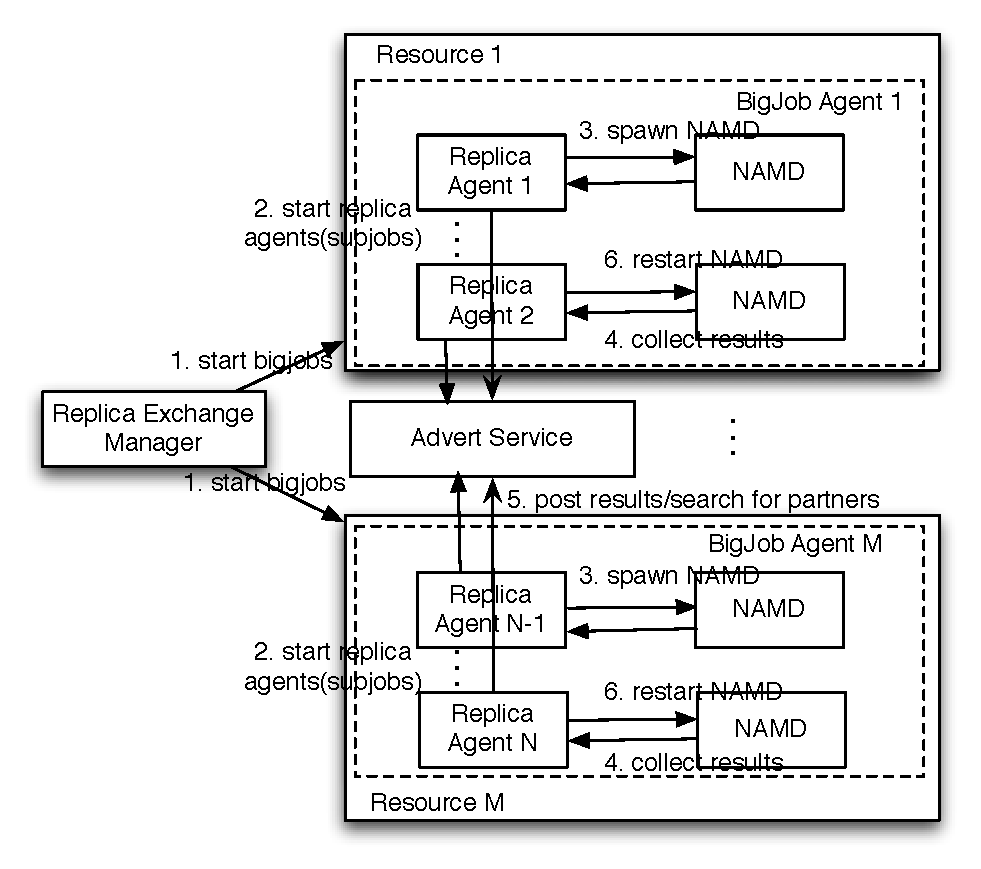
\includegraphics[width=0.9\textwidth]{asyncre.pdf}
% %\label{fig:async:b}
% \caption{\small Decentralized control flow: In the decentralized asynchronous RE, for  each replica there is a replica-agent which individually manages the replica.}
% \label{fig:decent}
% %\vspace{-1em}
% \end{figure}

%\alnote{we should write Case consistently with small or capital letter}
% We have to bear in mind that while Case II and Case III both implement the same asynchronous RE algorithm, they do it differently.
% At first glance it appears to be a question of philosophy, whether to
% let the replicas be managed by a master or to let each replica be
% managed individually.
%There could be implications effecting the performance of the
%algorithm. Where as in Case II, the master has to manage all the
%replicas and since it can only manage one replica at a time, although negligible, it is a cause for concern with large number of replicas. %The effect could be negligible and might now effect the overall performance.
%But the decentralized version (Case III) has no
%such issues as each replica is managed individually. % \jhanote{The distinction between Case 3 and 2 needs to
%  be made more clear. The following is ``implementation detail''. What
%  is the conceptual difference between Case 3 and Case 2?}

\section{Scale-Up and Scale-Out: Experiments and Results}
\label{sec:performance}

To evaluate the scale-up and scale-out properties of the different RE
algorithms and implementations, we conducted several experiments on TG
and LONI resources. By ``scale-up", we mean increasing the number of
replicas while keeping the number of machines constant and by
``scale-out", we mean increasing the number of machines while keeping
the number of replicas constant.  In this section we detail the
experiments that were conducted, the experimental results and the
analysis.

% \alnote{Should we reference the model used? Not sure which model it is
%   Hepatitis or HIV?}

%
%%%%% FIGURE %%%%%
\begin{figure}
\centering
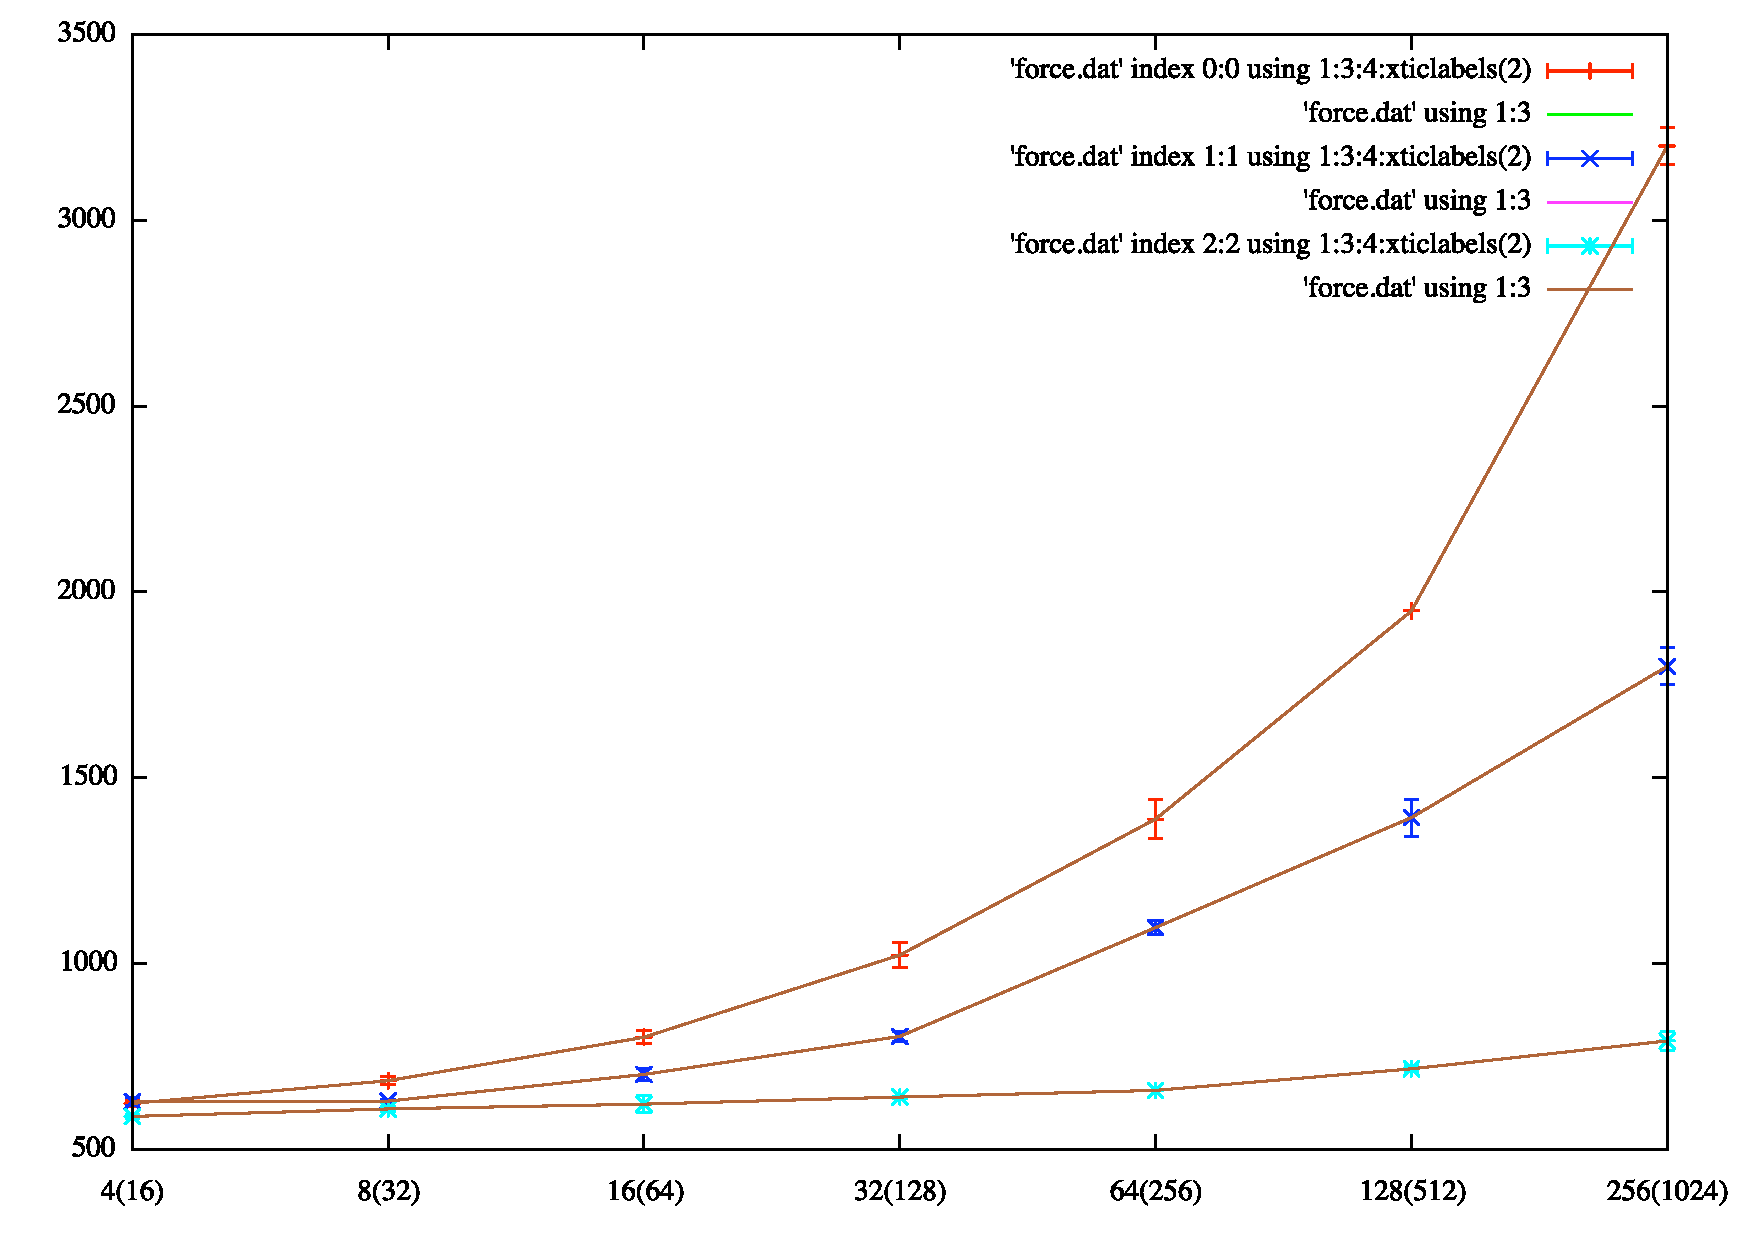
\includegraphics[width=0.9\textwidth]{../data/scale_up_gnu.pdf}
\caption{\small \textbf{Scale-Up Performance for 8 to 256 Replicas:}
  The graph shows the runtimes for the different RE implementations.
  The asynchronous decentralised RE implementation shows the best
  scaling behaviour. Both centralised RE versions scale less well
  mainly due to the limitations of the single master, which becomes a
  bottleneck.}
\label{fig:scaleup}
\alnote{The notation of the x- and y-label is kind of confusing. On
  the y-axis the unit is in parentheses. On the x-axis
  \#exchanges. Since we keep the ratio between \#replica and
  \#attempted exchanges constant, do we need both values on the
  x-axis?}  \vspace{-1em}
\end{figure}

\subsection{Scale-Up}


{\it Experiments: }
We repeated each of the synchronous and asynchronous experiments with 4, 8, 16, 32, 64, 128 and 256 replicas making 16, 32, 64, 128, 256, 512 and 1024 exchanges, respectively, on one machine. Each replica is configured to run 500 time-steps and is allocated 16 processors. The experiments consisting up to 128 replicas are done on {\it QueenBee}, while the experiments with 256 replicas are done on \emph{Ranger} (this is because \emph{QueenBee} only allocates a maximum of 2048 processors per job request). But we have normalised the data from {\it Ranger} to compare with results from \emph{QueenBee}.
It should be noted that the ratio between the number of
replicas and attempted exchanges is kept constant, so that it allows for comparison between each of these experiments.

%\subsubsection{Scale up performance: Results and Analysis}

{\it Results:} Figure~\ref{fig:scaleup} shows the results obtained by
running the experiments mentioned previously.  As the number of
replicas increases, $T_{C}$ increases as well. This increase, however,
is not uniform across the three cases.  We see the most slow down in
case I and the least in case III.  \alnote{need to be aligned with sec
  4} The synchronous version (case I) shows the worst scaling
behaviour due to various reasons: as described in
section~\ref{sec:impl_sync_re}, $T_{W}$, i.\,e.\ the time spent
waiting for other replicas of a generation to finish, is the main
driver of this performance degradation. Since replicas are currently
started sequentially by the master, a delay between the start and thus
the termination of the first and last replica exists. Further,
different nodes of a machine tend to show a slightly different
performance. With more replicas, the time to start the replicas as
well as the synchronization time increases.  In case II, exchanges
happen in an asynchronous manner, but they are still orchestrated by
the master.  As the number of replicas increases, the master quickly
becomes a bottleneck. But in case III, the exchanges are all carried
out in a decentralised way, i.\,e.\ exchanges can occur concurrently
between different pairs of replicas. Therefore, it can be concluded
that the asynchronous RE algorithm scales better and that the
decentralised implementation is superior to the centralised one.

%
%%%%% FIGURE %%%%%
\begin{figure}%
\centering
\subfigure[8 replicas]{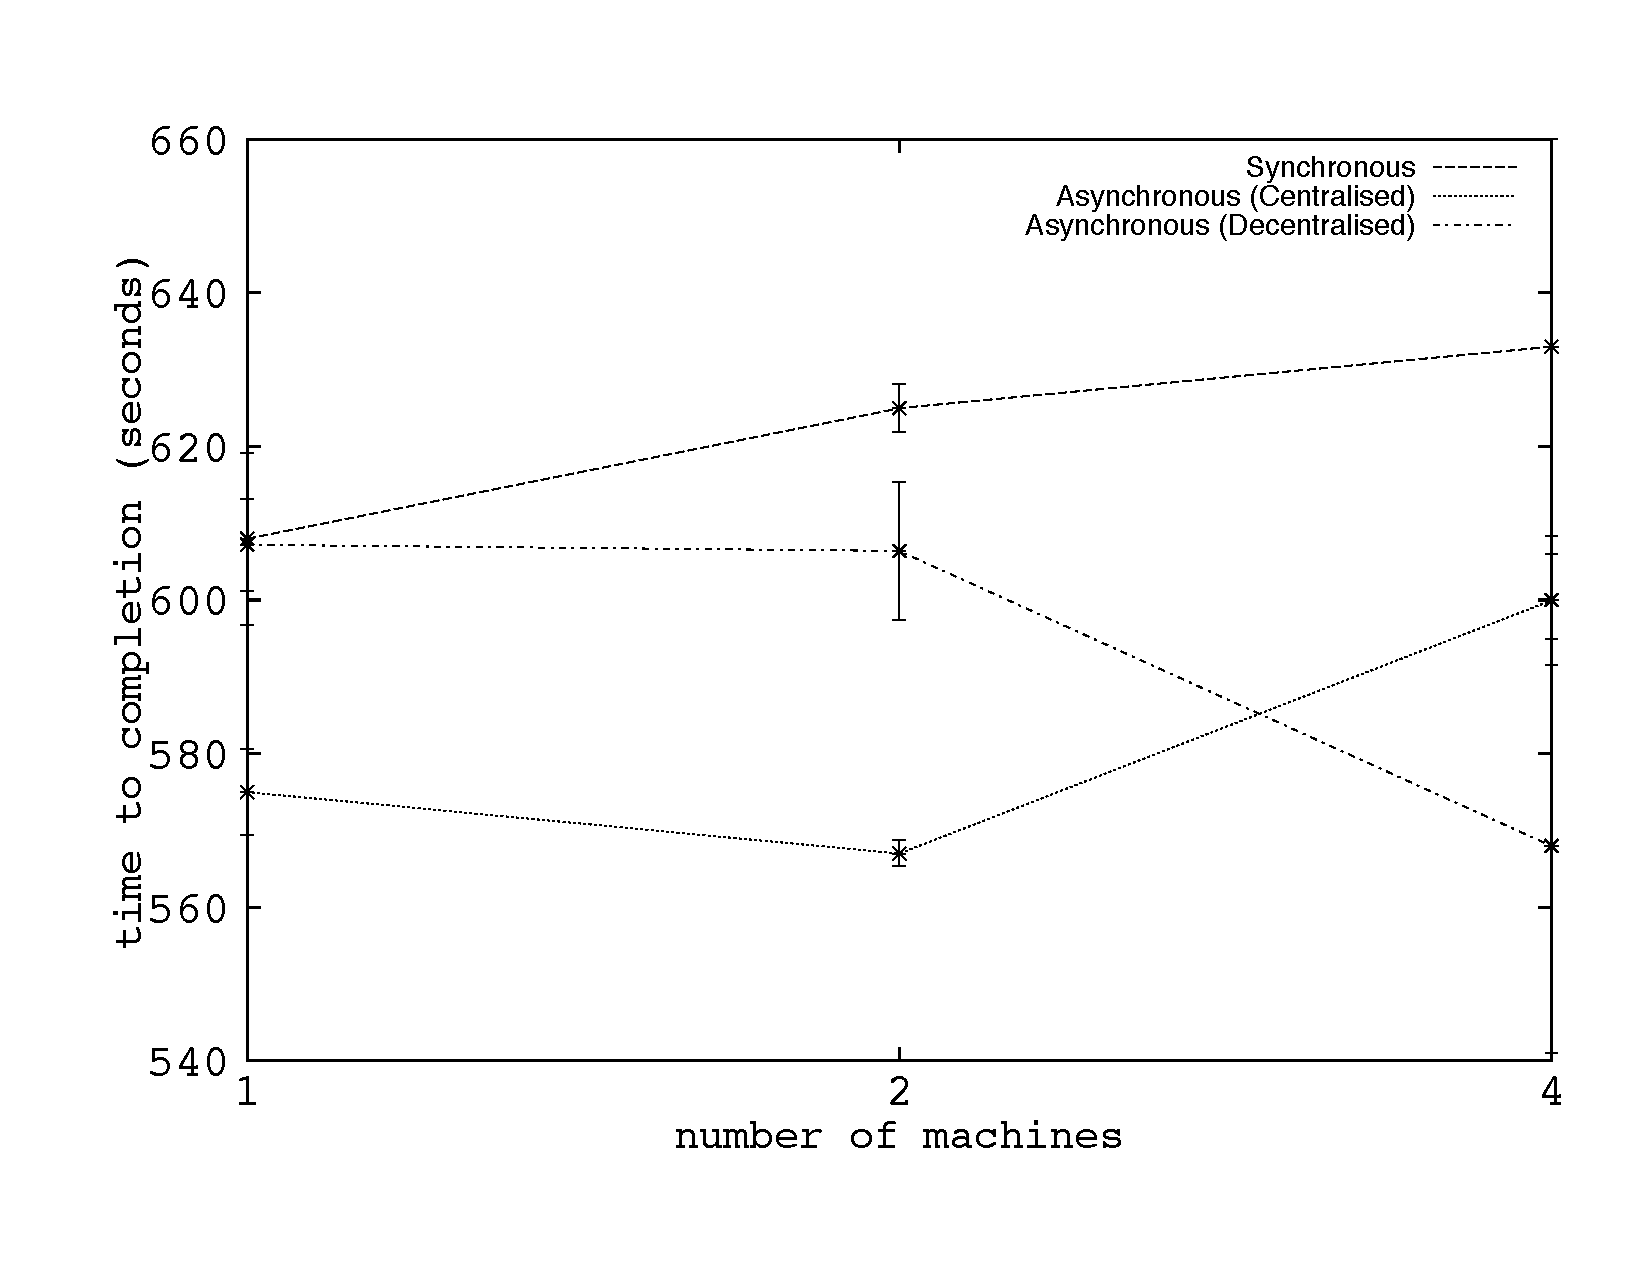
\includegraphics[width=0.47\textwidth]{../data/scaleout_8.pdf}}\qquad
% \subfigure[16 replicas]{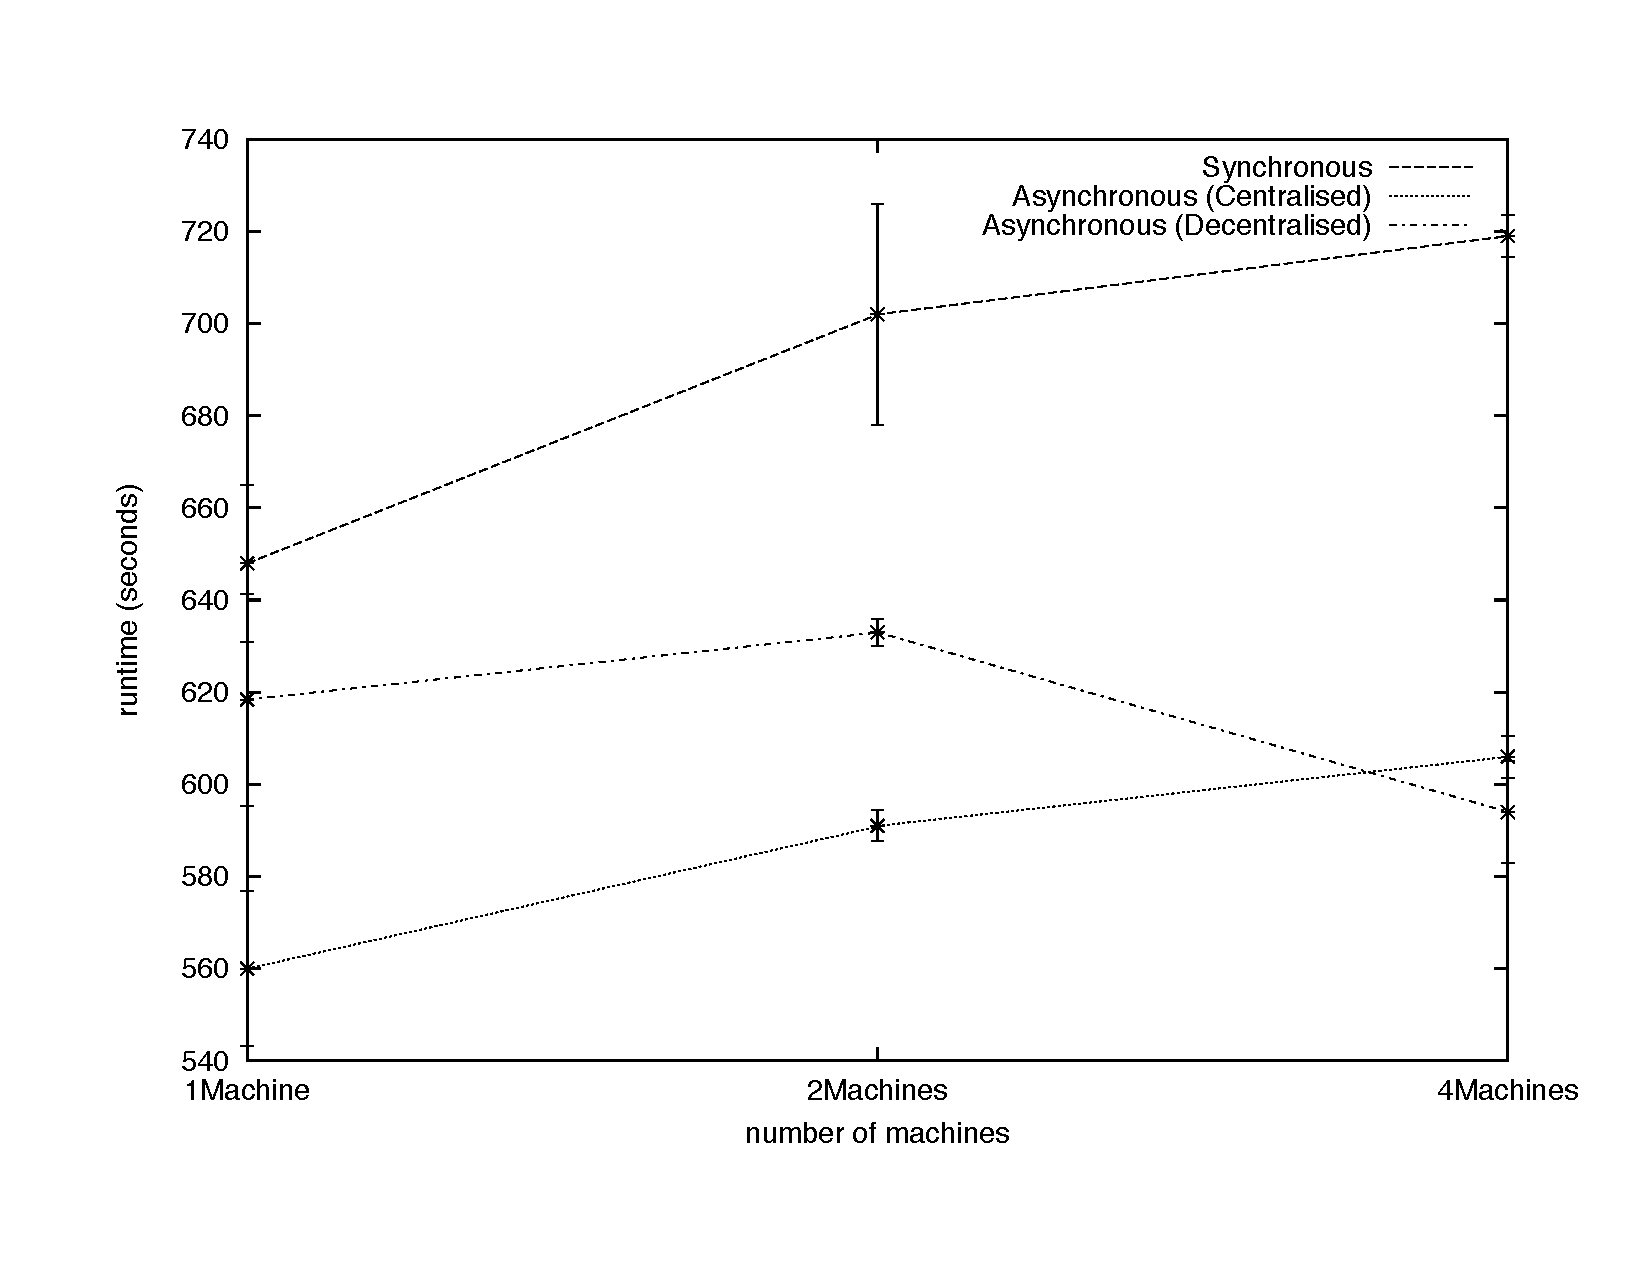
\includegraphics[width=0.55\textwidth]{../data/scaleo_16.pdf}}\\
\subfigure[32 replicas]{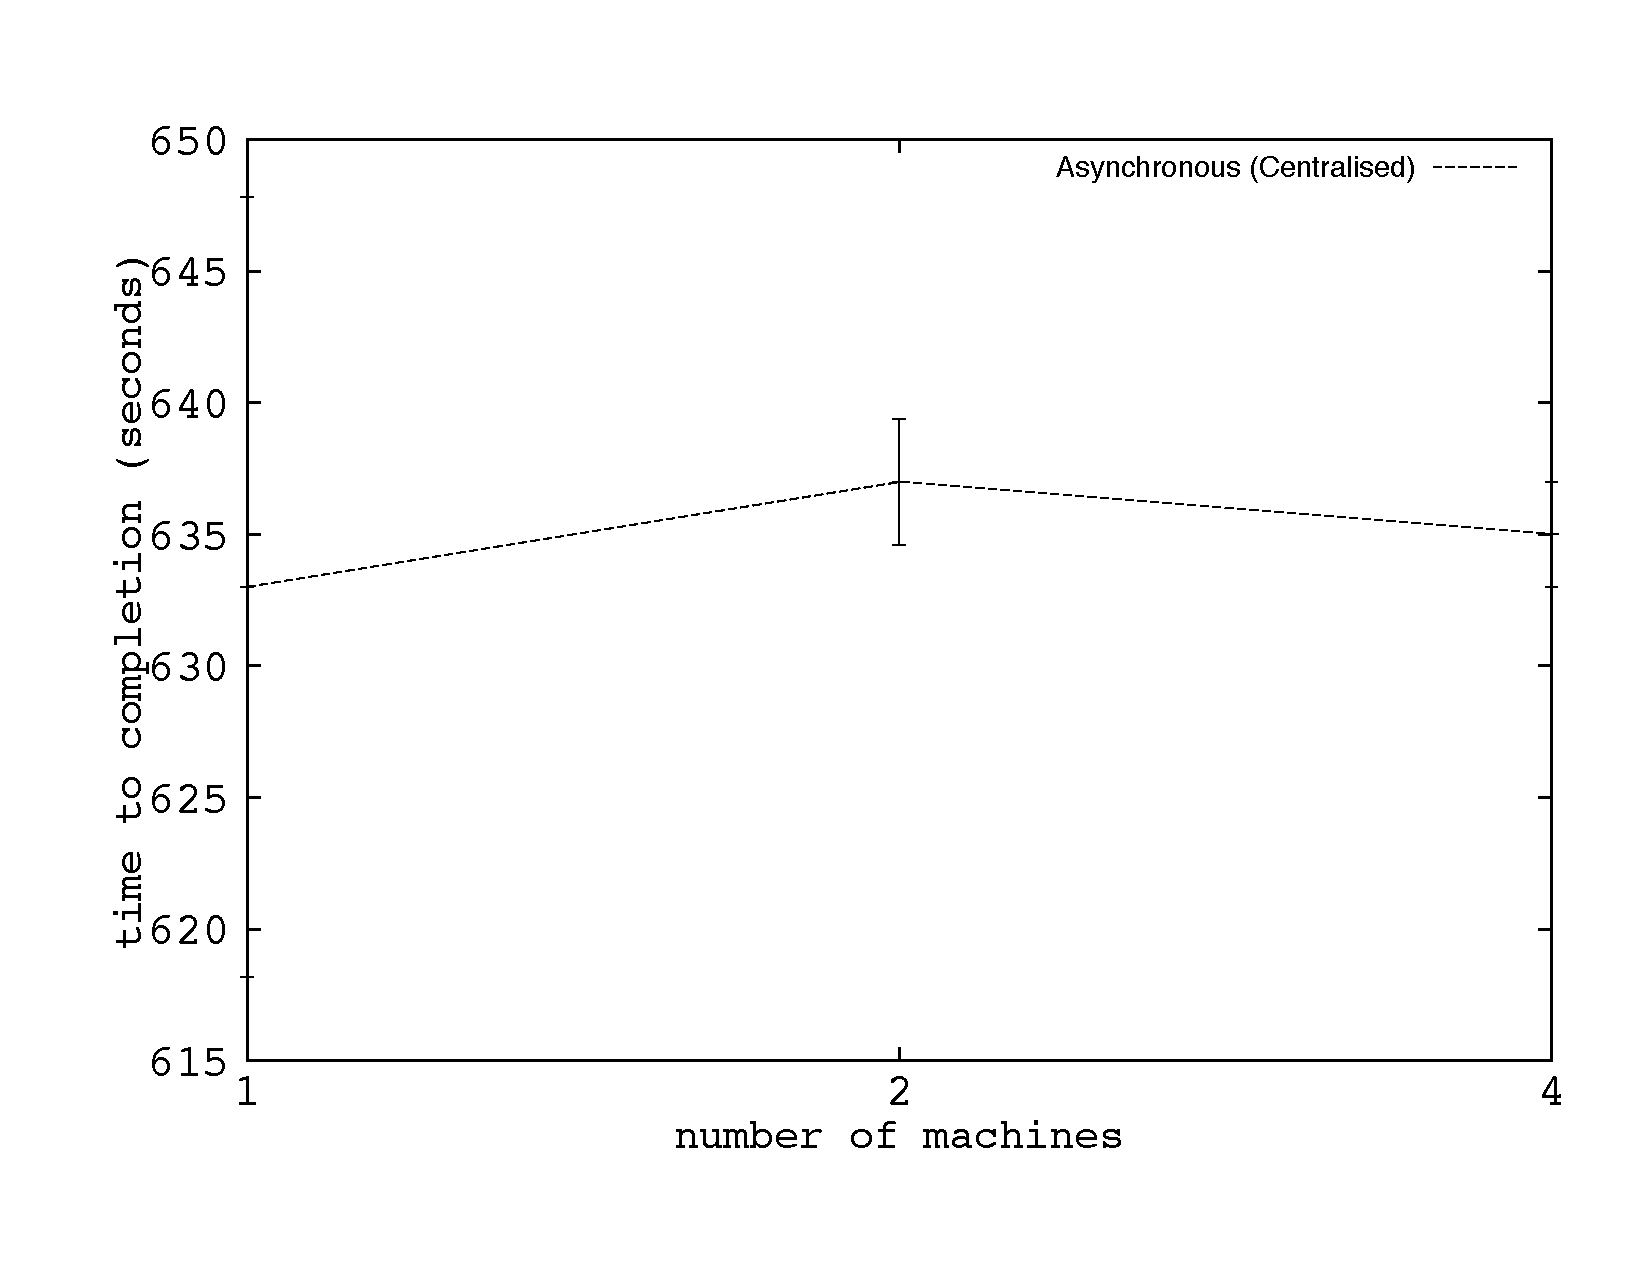
\includegraphics[width=0.47\textwidth]{../data/scaleout_32.pdf}}
\caption{\textbf{Scale-out Performance for 8, 16 and 32 Replicas:} 
  TBD.}
\alnote{16 or 32 replicas? Why is the centralised async performing
  better for 8 replicas and a small number of machines? We should
  consider showing only the 32 replica scenario. bar chart instead of
  lines? opinions?}  \alnote{Could you check the figures again. They
  look very pixelated. Further I would propose to just have numbers on
  the x-axis und not 1Machine, 2Machines,.... If otherwise, please use
  a space between 1 and machine.} \jhanote{the labels have to be made
  larger. Currently can't be read}
\label{fig:24machines}

\end{figure}

\subsection{Scale out}

{\it Experiments:} In this scenario we investigate the scale-out
behaviour of the three RE implementations. For this purpose we used
the following LONI and TG resources: QueenBee, Ranger, Abe,
?\alnote{Abhinav: could you please provide the machines used?}  We
utilised up to four machines concurrently running between 8 and 32
replicas. All experiments have been conducted using four big-jobs.
The replicas and big-jobs are evenly distributed across all
resources. Once all big-jobs became active, the replicas are assigned
to them by the RE-Manager. For all experiments we only consider the
runtime and not the queuing time at the local LRMS. \alnote{Is this
  correct? When do we start to assign the replicas? If the queue time
  is included, we had at least an explanation for the high stddev-}
\alnote{How many repeats?}\jhanote{LRMS.. Shouldn't we use batch-queue
  scheduler?}

{\it Results:} As seen in Figure~\ref{fig:24machines} the performance
of the synchronous RE implementation degrades significantly the more
resources are used.  In particular with a larger number of replicas
the asynchronous RE implementations performs very well. The
asynchronous-decentralised RE version shows as expected the best
performance.

\alnote{To-be-answered: Why is case II faster than III in the
  8rep/[1,2] machine scenario?}
% {\it Analysis: } 
The slowdown of the synchronous version is mainly caused by the
synchronization phase after each generation and the associated high
$T_{W}$ value. In a heterogeneous, distributed environment the
performance deteriorates even more since the slowest machine
determines the overall progress of the simulation. The asynchronous RE
versions do not have this limitation. As in the scale-up scenario, the
asynchronous-decentralised version performs better with a large number
of replicas mainly due to the fact that exchanges can be carried out
concurrently via the advert service without involvement of a central
coordinator.  \alnote{TODO: Local vs. distributed coordination, BigJob
  startup times}

% Overall, there is not much difference between the local and distributed 
% runs in any case. The reason being that there is very
% little interaction between the replicas. A very small configuration
% file is staged to the remote machines after an exchange, which will
% not add more than a couple of seconds per exchange. The rest of the
% co-ordination is done via the advert service, which is usually located
% on a remote machine in any case. Each query to the advert server is in
% the order of milli seconds and does not produce a noticeable effect on
% the performance.

% \subsubsection{Scale out performance: Results and Analysis}


%  In Figure~\ref{fig:24machines}, we see the performance
% of all three cases when run in a distributed manner across two
% machines. As the data that is exchanged between replicas is very
% small, the cases I, II and III behave in a similar manner to the way
% they behave on a single machine. \alnote{we should add some numbers
%   and maybe a graph for an example scenario: x: machines y:
%   time-to-solution} Again, asynchronous RE is better suited for
% distributed runs and the decentralised implementation scales best. The
% reason is, since each replica has its own replica-agent, there is no
% need to transfer any files between machines. The required
% configuration files are created locally by the replica-agent.


%In Case I, the pair-wise replica exchange can occur only between replicas of the same generation. Therefore, each exchange step is attempted only after all the replicas have finished running. After the exchange, all the replicas are restarted sequentially. This inserts a delay between the start time of the first replica, the last replica and the replicas in between. %As more resources become available at different times, the replicas already running or done are forced to wait for the newly running replicas to finish before moving on to the next exchange step. %Each exchange step is counted as an exchange.
%In Case II, the pair-wise replica exchange can take place between any two replicas in the ensemble irrespective of generation. As more resources become available, the new replicas join the ensemble immediately and the replicas already running are not restrained from attempting exchanges or restarting. This gives the asynchronous or synchronous RE a slight advantage. But with a large number of replicas we could easily see large difference.
%\athotanote{Further, we show performance gains by running across more than one machine. By running across more than one machine, we demonstrate the ability to divide the jobs into smaller sub-jobs and then distribute them across a number of machines, thereby reducing the risk of long queue wait times on an over-crowded resource. In Figure~\ref{fig:graph}, it can be seen that the asynchronous RE time to completion improves almost by a factor of 3 when moving from one machine to four machines. This was caused due to the fact that when the experiment was done on one machine, by the time the experiment ended, only 64 cores were allocated by the resource manager. But on the other hand, when the experiment was launched across four machines, it received an allocation of 64 cores on each of the four resources. The improvement that is seen in the case of synchronous RE from one to four machines is also due to a similar reason.} %The asynchronous RE appears faster by a couple of minutes due to the fact that when the BigJobs become available randomly, the synchronous RE has to wait for the newly running replicas to finish.

%slightly over 2 machines, but again increases over 4 machines. This is due to the fact that the experiments have been run only a handful of times but, over time, it can be assumed that it will result in reduced queue wait times.

\section{Conclusion}
\label{sec:conclusion}


%\athotanote{is this right? }
% We are also going to have a wider group of replicas to look at for
% each replica as we are not pairing the replicas.

% Also, we have the usual advantages of using a pilot-job,
% such as reduced queue wait times by not having to submit to the queue
% at every step.  We also provide major advantages when compared to
% Parashar et al.

%  to run the asynchronous RE simulations,
% including the ability to run MPI
% jobs.
% ??We need to evaluate the performance of our models and compare with other models for conducting replica exchange simulations.


%%%%% FIGURE %%%%%
%\begin{figure}
%\centering
%\subfigure[Time to complete 64 exchanges on QB with two 64 core BigJobs and on both QB/Louie jointly with a 64 core BigJob on each machine.]{
%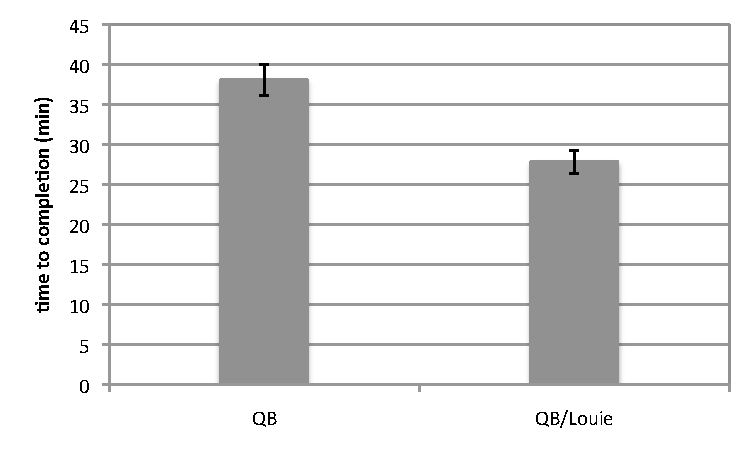
\includegraphics[width=0.40\textwidth]{figures/graph1.pdf}
%\label{fig:subfig3}
%}
%\hspace{0.5cm}
%\subfigure[Time to complete different number of exchanges on QB/Louie with a 64 core BigJob on each machine.]{
%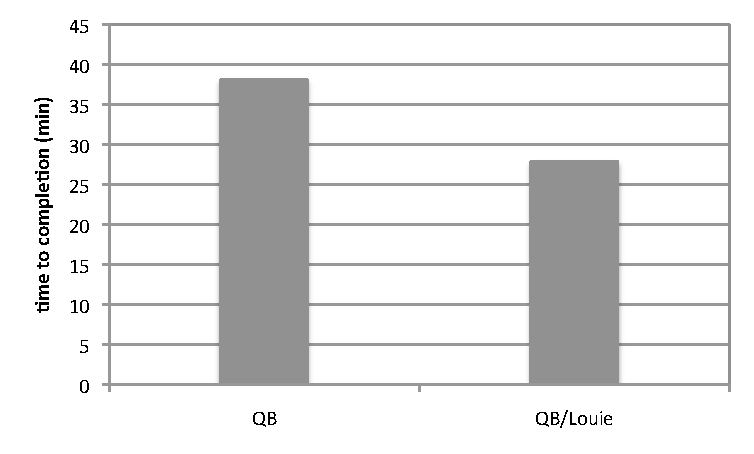
\includegraphics[width=0.40\textwidth]{figures/graph2.pdf}
%\label{fig:subfig4}
%}
%\caption{\small In Figure 2(a), we can see the improvement in performance when run on more than one machine. It is due to the fact that usually the first queued job becomes active before the second on a machine and running jobs on more than one machine solves this problem. In Figure 2(b), we can see consistent performance over prolonged runs, making 32, 64 and 128 exchanges.}
%\label{fig:graphs}
%\vspace{-1em}
%\end{figure}
%%%%% FIGURE %%%%%

An important motivation for this work is to implement a scheme that does not depend on a
static, well defined model of resource availability. %We test and scale
%our implementation on production level grids such as Teragrid and
%LONI~\citep{LONI_web}.
Preliminary results, shown in Figure~\ref{fig:graph}, indicate the
most important advantages of asynchronous RE and SAGA/BigJob over
traditional RE: (a) allows for exchanges to occur between replicas
with non-nearest temperatures, which in turn allows crosswalks to
happen (b) a reduced time to completion when running on more than one
machine due to improved resource availabilities, (c) the advantage of
using a pilot-job mechanism, which eliminates the waiting times at the
local resource manager, \alnote{have shown this in prev. papers, but
  we don't really have data in this one} and (d) the ability to scale
out across different production level infrastructure, such as, the
Teragrid and LONI.
% It performs well even after doubling and quadrupling the number of
% exchanges required to complete the simulation. The time to
% completion only increases by 35\% after doubling and 117\% after
% quadrupling the number of exchanges.
%\athotanote{should the results
%  be included in the conclusion or in a separate results section? Do
%  you agree with the \# of exchanges scheme to show the data?}
% Unfortunately we have results only for Case II currently, but 

%In summary, we have established the ability to scale-out across different
%infrastructure and compared the performance of the asynchronous
%RE with the synchronous RE at large scales. 
Further, we compare the traditional RE model (case I) and the centralised (case II) and decentralised (case III) models of the asynchronous replica exchange by modeling and repeating the experiments a reasonable number of times, so as to accurately quantify the scientific and performance gains. %We also propose to measure the frequency with which crosswalks occur with increasing number of replicas and measure the advantages due to a decentralized implementation in the full paper.


%With this asynchronous replica exchange mechanism we can improve the
%number of exchanges per unit time, a key parameter in judging the
%performance of a replica-exchange mechanism. \athotanote{is this
 % right? }  We are also going to have a wider group of replicas to
%look at for each replica as we are not pairing the replicas. Also, we
%have the usual advantages of using a pilot-job, such as reduced queue
%wait times by not having to submit to the queue.  Unfortunately we
%dont have results \jhanote{What results can we present -- any? some?},
%so we will say, (i) we establish the ability to scale-out (distributed
%and exa-scale) across different infrastructure (ii) compare the Async
%versus sync formulation at unprecedented scales \jhanote{At least
%  outline what infrastructure we / you are planning to use?} (iii)
%compare different implementations of the Async version
 

\begin{acknowledgement}
  This work is part of the Cybertools (http://cybertools .loni.org)
  project and primarily funded by NSF/LEQSF (2007-10)-CyberRII-01.
  Important funding for SAGA has been provided by the UK EPSRC grant
  number GR/D0766171/1 (via OMII-UK) and HPCOPS NSF-OCI 0710874. This
  work has also been made possible thanks to computer resources
  provided by TeraGrid TRAC TG-MCB090174 and LONI resources.
\end{acknowledgement}

\bibliographystyle{kluwer}
\bibliography{saga,literature}    
\end{document}


% and $T_W=T_w+T_r$, and where
%($T_w$), 

% \begin{eqnarray}
% T = {1\over p} \times [(T_{MD} \times  {N_X \over {N_R \over 2}}) + (T_{X} + T_{W}) \times N_X]
% \label{eq:totaltime}
% \end{eqnarray}

% \alnote{Using ex and EX as subscripts is very
%   confusing!} \jhanote{Why not use T$_X$ in lieu of $T_{EX}$? }

% Equation \ref{eq:totaltime} gives the total time to complete an RE
% experiment. The next equation aims to calculate the time to complete
% particular number of exchanges ($N_z$), where $0 \geq N_z \geq N_X$.

% \begin{eqnarray}
% T_z = {1\over p} \times [(T_{MD} \times  \lceil{N_z \over {N_R \over 2}}\rceil) + (T_{EX} + T_{W}) \times N_z]
% \label{eq:parttime}
% \end{eqnarray}

% Here $\lceil$ $\rceil$ denotes the ceiling function. The reason we put the term ${N_z \over {N_R \over 2}}$ under a ceiling function is because the ensemble of replicas run concurrently and for each concurrent run, $N_R \over 2$ exchanges are possible. Therefore, only the coordination and waiting costs effect the total time. 

% \athotanote{please suggest alternative terms if you find anything
%   confusing}

%It should be noted that only the coordination and waiting costs are divided by $\eta$. The ensemble of replicas are already running concurrently and 


% The RE algorithm involves the concurrent execution of multiple similar
% simulations, the \emph{replicas}.  There is a loose-coupling between
% the replicas in form of periodic exchange attempts between paired
% replicas. The traditional approach to RE is the synchronous model,
% which works well in an ideal scenario with a well defined model of
% resource availability. But with heterogenous systems and fluctuating
% resource availability, the asynchronous RE model could be more
% effectively used to conduct simulations. 
% >>>>>>> .r3441


%Previously, we demonstrated the usage of the SAGA Pilot-Job
%framework~\citep{saga_bigjob_condor_cloud} -- called the BigJob, to run
%RE simulations across multiple, heterogeneous distributed Grid and
%Cloud infrastructures~\citep{Luckow:2008fp}.
%\alnote{maybe we should also intro SAGA at some point} \jhanote{Yes} The Simple API for Grid Applications (SAGA)~\citep{saga_gfd90} is an API standardization effort within the Open Grid Forum (OGF)~\citep{ogf_web}, an international standards development body concerned primarily with standards for distributed computing. The various tasks that are carried out using the SAGA APIs include file staging, job spawning and the conduction of the exchange attempts.
%Further, we introduced several adaptivity modes, e.\,g.\ adaptive
%sampling that are able to react to dynamic changes in resource
%availabilities.

%\alnote{Not sure how many technical we need to provide...}  

%Traditionally, depending
%on the number of processes \texttt{N}, the manager creates \texttt{N/2} pairs
%of replicas.  Before launching a job, the manager ensures that all
%required input files are transferred to the respective resource. For
%this purpose, the SAGA File API and the GridFTP adaptor are used. The
%replica jobs are then submitted to the resource using the SAGA CPR
%API and the MIGOL/GRAM middleware.

%\jhanote{Mention that these are SAGA-based implementations. Something  else would be implemented differently}
%\alnote{Proposed structure: a) math. model b) sync c) async. We should give the reader some orientation in this section.}
% \jhanote{Abhinav: I still note the inconsistent and variable use of
%   algorithms, methods(?) and cases/approaches. I think we should refer
%   to Replica-Exchange as a ``class of algorithms'' or ``algorithm'',
%   and different implementations -- sync versus async} 

% \athotanote{RE class of algorithms - synchronous and asynchronous
%   models within RE class of algorithms; later sync, centralized-async,
%   decent-async implementation. right? or - RE class of algorithms -
%   synchronous and asynchronous implementation of RE class of
%   algorithms; later sync, centralized-async, decent-async
%   implementations. please suggest.}  \jhanote{I would say (i) RE Class
%   of Algorithms, (ii) Sync/Async algorithms too, and then centralized
%   or decentralized implementations of these sync versus async RE
%   algorithm}
%\subsection{Mathematical Model}
%\alnote{I think we should discuss the mathematical model before going
%  into the specifics of sync/async RE.}
%Here we first provide a basic mathematical model for different RE
% models which explains the terms involved. In this section, we aim to
% develop an equation for total time to run any RE simulation. If $t$
% is the average time between successful exchanges, and $p$ is the
% probability of a successful exchange,
%\begin{eqnarray}
%t=  {1 \over p} \times {[T_{MD} + T_{X} + T_{W}]} 
%\label{eq:timebtw}
%\end{eqnarray}
%where $T_{X}$ is the time to carry-out a pairwise exchange, which is
%comprised of (i) finding a partner, (ii) exchanging states including
%file transfer, (iii) book-keeping, and (iv) (re)starting the replica;
%$T_{W}$ is the time spent waiting for all replicas to complete running.
%Therefore, ${T_{X}} = {T_F + T_{ex} + T_{coord}}$ 
%and for ${T_{X}}^{async}, T_W = 0$
%The time ($T$) for N$_{X}$ exchanges is therefore $N_{X} \times t$
%If there are $\eta$ independent exchange events occurring
%concurrently, then the time $T$ for N$_x$ exchanges is $T \over \eta$.
